% mn2esample.tex
%
% v2.1 released 22nd May 2002 (G. Hutton)
%
% The mnsample.tex file has been amended to highlight
% the proper use of LaTeX2e code with the class file
% and using natbib cross-referencing. These changes
% do not reflect the original paper by A. V. Raveendran.
%
% Previous versions of this sample document were
% compatible with the LaTeX 2.09 style file mn.sty
% v1.2 released 5th September 1994 (M. Reed)
% v1.1 released 18th July 1994
% v1.0 released 28th January 1994

\documentclass[useAMS,usenatbib]{mn2e}
\usepackage[T1]{fontenc}
\usepackage{prettyref}
\usepackage{amsmath}
\usepackage{graphicx}
\usepackage{subfigure}
\usepackage{epstopdf}
\usepackage{color}
\usepackage[breaklinks=true]{hyperref} 

% If your system does not have the AMS fonts version 2.0 installed, then
% remove the useAMS option.
%
% useAMS allows you to obtain upright Greek characters.
% e.g. \umu, \upi etc.  See the section on "Upright Greek characters" in
% this guide for further information.
%
% If you are using AMS 2.0 fonts, bold math letters/symbols are available
% at a larger range of sizes for NFSS release 1 and 2 (using \boldmath or
% preferably \bmath).
%
% The usenatbib command allows the use of Patrick Daly's natbib.sty for
% cross-referencing.
%
% If you wish to typeset the paper in Times font (if you do not have the
% PostScript Type 1 Computer Modern fonts you will need to do this to get
% smoother fonts in a PDF file) then uncomment the next line
% \usepackage{Times}

%%%%% AUTHORS - PLACE YOUR OWN MACROS HERE %%%%%

\title[Predictions of Stellar Occulations by irregular satellites]{Stellar occultation predictions for 10 irregular satellites of giant planets plus Triton for 2016-2017}

\author[A. R. Gomes-Júnior, M. Assafin, L. Beauvalet et al.]{
A. R. Gomes-Júnior$^{1}$\thanks{E-mail: altair08@astro.ufrj.br},
M. Assafin$^{1,\dag,\ddag}$\thanks{E-mail: massaf@astro.ufrj.br},
L. Beauvalet$^{2,3}$,
R. Vieira-Martins$^{1,2,\dag,\ddag}$,
J.I.B. Camargo$^{2,\dag}$,
J. Desmars$^{4}$
B. E. Morgado$^{1,2}$
F. Braga-Ribas$^{2, 5, \dag}$,
\\
$^{1}$Observat\'orio do Valongo/UFRJ, Ladeira Pedro Ant\^onio 43,
CEP 20.080-090 Rio de Janeiro - RJ, Brazil\\
$^{2}$Observat\'orio Nacional/MCTI, R. General Jos\'e Cristino 77, CEP 20921-400 Rio de Janeiro - RJ, Brazil\\
$^{3}$Observatoire de Paris/SYRTE, 77 Avenue Denfert Rochereau 75014 Paris, France\\
$^{4}$Institut de mécanique céleste et de calcul des éphémérides - Observatoire de Paris, UMR 8028 du CNRS,
77 Av. Denfert-Rochereau, 75014 Paris, France\\
$^{5}$Federal University of Technology - Paran\'a (UTFPR / DAFIS), Rua Sete de Setembro, 3165, CEP 80230-901, Curitiba, PR, Brazil\\
$^\dag$ Associated to Laborat\'{o}rio Interinstitucional de e-Astronomia - LIneA, Rua Gal. Jos\'e Cristino 77, CEP 20921-400,\\ Rio de Janeiro, Brazil\\
$^\ddag$Affiliated researcher at Observatoire de Paris/IMCCE, 77 Avenue Denfert Rochereau 75014 Paris, France
}

\begin{document}

\date{Accepted . Received ; in original form }

\pagerange{\pageref{firstpage}--\pageref{lastpage}} \pubyear{2015}

\maketitle

\label{firstpage}

\abstract
Due to their orbital configurations, it is common belief that the irregular satellites were probably captured by the giant planets in the early solar system. It is important to know their physical parameters, such as size, shape, albedo and composition, to trace back their true origin. The best ground-based technique to determine size and shape, and thus constrain the albedo and in a broader sense composition, is the observation of stellar occultations by these objects.
We aim to predict stellar occultations for the eight largest irregular satellites of Jupiter: Himalia, Elara, Pasiphae, Carme, Lysithea, Sinope, Ananke and Leda, and for the irregular satellites Phoebe of Saturn and Nereid of Neptune, and also for Triton.
We identified candidates to stellar occultations by the irregular satellites from the UCAC4 catalogue and from a catalogue of stars in the sky-path of Neptune obtained from observations made with the ESO2p2/WFI (2.2 m Max-Planck ESO telescope with the Wide Field Imager) instrument. These catalogues were crossed with the ephemeris of the satellites to identify stellar occultations. We used a new ephemeris based solely on the observations from \cite{GomesJunior2015} to generate predictions for the short-time future or the satellites of Jupiter. For Phoebe, we used an updated ephemeris and for Nereid and Triton we used recently published ephemeris.
We managed to identify 396 candidates of stellar occultations between the period of January, 2016 and December, 2017. We made observational tests for the prediction of the event of Himalia in March 03, 2015. The stars and objects were observed close to the date predicted and in the same field to minimize errors and the obtained relative satellite-star positions were used to evaluate the predictions. We call attention for an occultation by Triton of a bright star (R=12.5) in October 5, 2017. The event can be observed from Europe and the east coast of USA and will be a good opportunity to access the current state of the atmosphere of the satellite.
The comparisons between the predictions and the observation tests show a good agreement. We discuss how the successful observation of a stellar occultation by these objects is quite possible and present some of those potential occultations.


\begin{keywords}
Occultations - Planets and satellites: general - Planets and satellites: individual: Jovian and Saturnian irregular satellites - Planets and satellites: individual: Triton
\end{keywords}

%\section{Introduction} \label{Sec: introducao} 
%
%Irregular satellites revolve around giant planets at large distances, on eccentric, highly inclined and frequently retrograde orbits. Because of these peculiar orbits, it is largely accepted that these objects did not form by accretion around of their planet, but were captured by their planets in the early solar system \citep{Sheppard2005}.
%
%There are several of capture mechanisms of objects by giant planets suggested in the literature. For example the Gas Drag in the primordial circumplanetary nebulae \citep{Sheppard2005} where the object would be affected by the gas drag and its velocity slowed down until it be captured by the planet. Another mechanism is called pull-down capture \citep{Sheppard2005}, where the mass of the planet would increase while the object was temporarily captured. 
%
%A mechanism based in the Nice model \citep{Morbidelli2005, Tsiganis2005, Gomes2005} was proposed by \cite{Nesvorny2007} and, in the specific case of Jupiter with the modern Nice model, by \citealp{Nesvorny2014}. In this scenario, during the early solar system instability, encounters between the outer planets occurred. These planetary encounters could exchange energy and angular momentum between planets and the objects nearby allowing the capture of irregular bodies by the giant planets. In this scenario, the survival rate of prior-LHB (Late Heavy Bombardment) satellites is very small.
%
%Another possible mechanism is the capture through collisional interactions \citep{Sheppard2005}. A collision between two small bodies in the Hill's sphere of the planet could generate fragmented objects and the dissipated energy could be such that some of these objects could be captured.
%
%Some of these objects are in dynamical groups with similar semi-major axis, eccentricities and inclinations, called families, similar to families found in the Main Asteroid Belt. These families may have been created by a parent body disrupted by collisions with comets or other satellites \citep{Nesvorny2004}. These collisions are more likely to have occurred during the LHB \citep{Gomes2005}.
%
%\cite{Nesvorny2003} studied the collision rates between irregular satellites and concluded that some satellites could have been removed by collision with a bigger satellite. The collision rate between satellites of the Himalia Group (Himalia, Elara, Lysithea and Leda, mainly), for instance, was found to be more than one during the solar system age suggesting that their current structure was originated by satellite-satellite collision.
%
%For Phoebe, ejected material from its surface caused by impacts could evolve due to Poynting-Robertson drag and collide with Iapetus causing the large variation in albedo observed on it \citep{Nesvorny2003}. Indeed, Cassini detected in Phoebe an absorption feature at 2.42 $\mu m$ (probably CN combinations) that was also detected in the dark side of Iapetus \citep{Clark2005}.
%
%The region of origin of these object is not well known. \cite{Grav2003} and \cite{Grav2007} showed that the irregular satellites from the giant planets have their colors and spectral slopes similar to C-, D- and P-type asteroids, Centaurs and trans-neptunian objects (TNOs) suggesting that they come from different locations in the early solar system.
%
%In order to obtain precise fundamental physical parameters like size, shape and albedo for the irregular satellites and thus to contribute to the study of their origin, we want to observe stellar occultations, which provide  more accurate results than other ground-based techniques \citep{Sicardy2011, Ortiz2012, Braga-Ribas2014}.
%
%No observation of a stellar occultation by an irregular satellite was published up to date. Since their estimated sizes are very small (see Table \ref{Tab: satellite-diameter}), this may have prevented earlier tries. But, in fact, given their distances to us, current ephemeris and star positions are already good enough for the prediction of the exact location and instant where the shadow of the occultation will cross the Earth. For instance, Himalia, supposedly the largest irregular satellite of Jupiter has an estimated size of 150 km \citep{Porco2003}, which is equivalent to an apparent size of about 40 mas (milliarcseconds). Thus, in this case, the cumulated uncertainty of ephemeris and star position must be around 40 mas to get good chances of observing a stellar occultation, which is quite feasible today.
%
%\begin{table}
%\caption{\label{Tab: satellite-diameter} Estimated diameter of the satellites and correspondent apparent diameter}
%\begin{centering}
%\begin{tabular}{lccc}
%\hline  \hline
%\multicolumn{4}{c}{Diameter of the satellites} \tabularnewline
%Satellite  & mas\tablefootmark{a}  & km & References \tabularnewline
%\hline
%Ananke & 8 & 29 & 1 \tabularnewline
%Carme & 13 & 46 & 1 \tabularnewline
%Elara & 24 & 86 & 1 \tabularnewline
%Himalia & 41 & $(150\times120) \pm 20$\tablefootmark{b} & 2 \tabularnewline
%Leda & 5 & 20 & 1 \tabularnewline
%Lysithea & 10 & 36 & 1 \tabularnewline
%Pasiphae & 17 & 62 & 1 \tabularnewline
%Sinope & 10 & 37 & 1 \tabularnewline
%\hdashline
%Phoebe & 32 & $212 \pm 1.4$\tablefootmark{b} & 3 \tabularnewline
%\hdashline
%Nereid & 15 & $340 \pm 50$\tablefootmark{c} & 4 \tabularnewline
%Triton & 124 & $2707 \pm 2.0$\tablefootmark{c} & 5 \tabularnewline
%\hline
%\end{tabular}
%\tablebib{
%(1) \cite{Rettig2001}; (2) \cite{Porco2003}; (3) \cite{Thomas2010}; (4) \cite{Thomas1991}; (5) \cite{Thomas2000}.}
%\end{centering}
%\tablefoottext{a}{Using a mean distance from Jupiter of 5 AU, from Saturn of 9 AU and from Neptune of 30 AU.}
%\tablefoottext{b}{From Cassini observation.}
%\tablefoottext{c}{From Voyager-2 observation.}
%\par
%\end{table}
%
%From what we have just presented, we can think that the observation of an stellar occultation by an irregular satellite should be likelier than occultations by TNOs. The orbits of their host planets are well known and their observation time-span covers many orbital periods, contrary to TNOs.
%%Unlike stellar occultations by TNOs, which nevertheless have been proved effective, the observation of an occultation by a irregular satellite is, in principle, more favorable. The orbits of their host planets are well known and these satellites have been observed completing already many orbital periods around them, thus presenting better ephemeris than TNOs. 
%Moreover, the irregular satellites are closer to Earth which means a minor localization error in kilometer.
%
%\cite{GomesJunior2015} obtained 6523 suitable positions for 18 irregular satellites between 1992 and 2014 with an estimated error in the positions of about 60 to 80 mas. For some satellites the number of positions obtained is comparable to the number used in the numerical integration of orbits by the JPL \citep{Jacobson2012}. They pointed out that the ephemeris of the irregular satellites have systematic errors that may reach 200 mas for some satellites. For an object at the distance of Jupiter, this represents an error bigger than 700 km in the shadow path. Using the positions obtained by \cite{GomesJunior2015} we produced a specific ephemeris for short-time future for the satellites of Jupiter and better predict stellar occultations for these objects.
%
%We present in this paper stellar occultation predictions for the 8 major irregular satellites of Jupiter (Himalia, Elara, Pasiphae, Lysithea, Carme, Ananke, Sinope and Leda), Phoebe from Saturn and Nereid and Triton from Neptune. In the section \ref{Sec: Rationale} we explore the scientific rationale for the study of the irregular satellites and the possibility of having a common origin with TNOs. In section \ref{Sec: integration} we show the the process of the production of the new ephemeris. In section \ref{Sec: predictions}, we present the predictions of the stellar occultations by irregular satellites and how they were made. Some tests made to confirm the predictions are presented in section \ref{Sec: testes} and the final discussion are in section \ref{Sec: discussion}.
%
%\section{Scientific Rationale} \label{Sec: Rationale}
%
%%\textcolor{red}{Como pode ver, comparado ao paragrafo na Introducao que falou a respeito, o texto aqui está muito pequeno e chovendo no molhado.}
%
%%\textcolor{red}{Tem que falar mais. Citar o paper no livro da Barucci que voce me mostrou outro dia. Dar mais citacoes sobre essa hipotese. Falar dos albedos parecidos, cores. Tem que fundamentar a hipotese de irregulares = TNOs pequenos.}
%
%%\textcolor{red}{Tambem falar aqui das vantagens de se observar ocultacoes dos irregulares, porque apesar de alguns satelites terem efemerides ruins, outros nem tanto, as efemerides sao melhores que a de TNOs (os irregulares ja completaram voltas em torno dos seus planetas); no caso de Jupiter, ele esta proximo o que ajuda a diminuir o erro em km.}
%
%
%%\textcolor{red}{E dizer que, mesmo que a hipotese de TNOs que nos motiva a fazer as predicoes, venha a ser refutada no futuro, seja por outros trabalhos, seja pelos resultados futuros de observacoes de nossas proprias ocultacoes, o levantamento em si das propriedades fisicas, tamanho, forma e albedo ainda assim seriam muito uteis para testar as hiposteses de captura, ou seja, contribui para o estudo da formacao e evolucao dos sistemas de Jupiter, Saturno e Netuno.}
%
%There is no consensus for a single model explaining where the irregular satellites were formed. \cite{Cuk2004} showed that the progenitor of the Himalia group may have originated in heliocentric orbits similar to the Hilda asteroid group. \cite{Sheppard2005} stated that the irregular satellites may be some of the objects that were formed within the giant planets region.
%
%Phoebe is the most studied irregular satellite. \cite{Clark2005} suggest that its surface is probably covered by material of cometary origin. It was also stated by \cite{Johnson2005} that if the porosity of Phoebe is 15\%, Phoebe would have an uncompressed density similar to those of Pluto and Triton.
%
%\cite{Sheppard2005} and \cite{Jewitt2007} also expose the possibility for the irregular satellites having their origin as comets or TNOs. TNOs are highly interesting objects that, due to their large heliocentric distances, may be highly preserved having their physical properties similar to those they had when they were formed \citep{Camargo2014}. This is even more true for the smaller objects, since in principle larger sizes favour physical differentiation processes in the body and vice-versa. However, due to the distance, the smaller TNOs from this region are more difficult to observe. A clever way to overcome this difficulty is to study  the much closer irregular satellites, under the hypothesis that they share a common origin with the small TNOs' population.
%
%Triton is a uncommon satellite. Its orbit is retrograde and inclined, but quasi-circular and very close to the planet compared to the irregular ones. Because Triton's orbit size is very small and its precession is not dominated by Solar perturbations, Triton is frequently excluded from the irregular satellites' class, but studied together by many authors \citep{Sheppard2005, Jewitt2007}. 
%
%Similarly to the irregular satellites, Triton was probably captured in the early solar system and may have the same origin as the TNOs \citep{Agnor2006}. Differently, Triton is bigger than the irregular satellites by an order of magnitude and has an atmosphere. The main motivation to study Triton by stellar occultations is to understand the evolution of its atmosphere due to Triton's complicated and extreme seasonal cycle \citep{McKinnon2007}.

%Because they are faint, the majority of these objects was discovered only in the last century\footnote{Website: http://ssd.jpl.nasa.gov/?sat\_discovery} . They were never visited by a spacecraft, with the exception of Himalia, Phoebe and Nereid, in a flyby by the Cassini space probe in 2000 for Himalia \citep{Porco2003} and in 2004 for Phoebe \citep{Desmars2013} and in a flyby by the Voyager 2 space probe in 1989 for Nereid \citep{Smith1989}. Even in situ, they were still opportunity target observations resulting in not optimal measurements, with size errors of $10 km$ for Himalia and $25 km$ for Nereid \citep{Thomas1991}. The exception is Phoebe with a very accurate measurement of size with a mean radius error of $0.7 km$ \citep{Thomas2010}.

%If these objects were captured, there remains the question of where they came from. \citealp{Clark2005} showed from imaging spectroscopy from Cassini that Phoebe has a surface probably covered by material from the outer solar system and \citealp{Grav2003} showed that the satellites of the Jovian Prograde Group Himalia have grey colors implying that their surfaces are similar to that of C-type asteroids. In that same work, the Jovian Retrograde Group Carme was found to have surface colors similar to the D-type asteroids like Hilda or Trojan families while JXIII Kalyke has a redder color like Centaurs or trans-neptunian objects (TNOs).

%For Saturnian satellites, \citealp{Grav2007} showed by their colors and spectral slopes that these satellites contain a more or less equal fraction of C-, P- and D-like objects but SXXII Ijiraq is marginally redder than D-type objects. These works may suggest different origins for the irregular satellites.

%In this context, we used 3 databases for deriving precise positions for the irregular satellites observed at Observatório do Pico dos Dias (1.6 m and 0.6 m telescopes, IAU code 874), Observatoire Haute-Provence (1.2m telescope, IAU code 511) and ESO (2.2 m telescope, IAU code 809). Many irregular satellites were observed between 1992 and 2014 covering a few orbital periods of these objects (12 satellites of Jupiter, 4 of Saturn, Sycorax of Uranus and Nereid of Neptune). 

%Since their ephemerides are not very precise, predict and observe stellar occultations are very difficult and no observation of such an event for an irregular satellite is found in the literature. The precise star positions to be derived by the ESA astrometry satellite Gaia \citep{deBruijne2012} will render better predictions with the only source of error being the ephemeris. The positions derived from \textbf{our} observations can be used in new orbital numerical integrations, generating more precise ephemerides.

%The power of stellar occultations for observing relatively small diameter solar system objects is supported by recent works such as the discovery of a ring system around the Centaur (10199) Chariklo \citep{Braga-Ribas2014}. Once irregular satellites start to be observed by this technique, it will be possible to obtain their physical parameters (shape, size, albedo, density) with unprecedented precision. For instance, in this case, sizes could be obtained with kilometer accuracy. The knowledge of these parameters would in turn bring valuable information for the study of the capture mechanisms and origin of the irregular satellites.

%The databases are described in Sect. \ref{Sec: observations}. The astrometric procedures in Sect. \ref{Sec: reduction}. The obtained positions are presented in Sect \ref{Sec: positions} and analysed in Sect. \ref{Sec: comparison}. Conclusions are given in Sect. \ref{Sec: conclusions}.


\section{Introduction}\label{Sec: introducao}

Irregular satellites revolve around giant planets at large distances in eccentric, highly inclined and frequently retrograde orbits. Because of these peculiar orbits, it is largely accepted that these objects did not form by accretion around their planet, but were captured in the early solar system \citep{Sheppard2005}.

There is no consensus for a single model explaining where the irregular satellites were formed. \cite{Cuk2004} showed that the progenitor of the Himalia group may have originated in heliocentric orbits similar to the Hilda asteroid group. \cite{Sheppard2005} stated that the irregular satellites may be some of the objects that were formed within the giant planets region.

\cite{Grav2003} and \cite{Grav2007} showed that the irregular satellites from the giant planets have their colors and spectral slopes similar to C-, D- and P-type asteroids, Centaurs and trans-neptunian objects (TNOs). This suggests that they may have come from different locations in the early solar system.

\cite{Sheppard2005} and \cite{Jewitt2007} also explored the possibility that the irregular satellites originated as comets or TNOs. TNOs are highly interesting objects that, due to their large heliocentric distances, may be highly preserved with physical properties similar to those they had when they were formed \citep{Barucci2008}. This is even more true for the smaller objects, since in principle larger sizes favour physical differentiation processes in the body and vice-versa. However, due to the distance, the smaller TNOs from this region are more difficult to observe. Thus, if irregular satellites - or at least a few of them - do share a common origin with small TNOs, and since these objects are situated at much closer heliocentric distances now, this gives a unique chance of observing and studying representatives of this specific TNO population in much greater detail than could ever be possible by direct observation of this population in the Kuiper Belt. 

Phoebe is the most studied irregular satellite. \cite{Clark2005} suggest that its surface is probably covered by material of cometary origin. It was also stated by \cite{Johnson2005} that if the porosity of Phoebe is 15\%, Phoebe would have an uncompressed density similar to those of Pluto and Triton.

In order to obtain precise fundamental physical parameters like size and shape, thus constraining the albedo and in a broader sense also the composition for the irregular satellites and therefore to contribute to the study of their origin, we aim at observing stellar occultations, which provide  more accurate results than other ground-based techniques \citep{Sicardy2011, Ortiz2012, Braga-Ribas2014}. For that, reliable predictions of stellar occultations by these satellites are most needed.

We present in this paper stellar occultation predictions for the 8 major irregular satellites of Jupiter (Himalia, Elara, Pasiphae, Lysithea, Carme, Ananke, Sinope and Leda), Phoebe of Saturn and, Nereid and Triton of Neptune. Phoebe, being the most studied object with a good measured size, can be used to calibrate and evaluate the technique for similar objects.

Triton is an uncommon satellite. Its orbit is retrograde and inclined, but quasi-circular and very close to the planet compared to the irregular ones. Because Triton's orbit size is very small and its precession is not dominated by Solar perturbations, Triton is frequently excluded from the irregular satellites' class, but still studied together by many authors \citep{Sheppard2005, Jewitt2007}. Similarly to the irregular satellites, Triton was probably captured in the early solar system and may have the same origin as the TNOs \citep{Agnor2006}. However, Triton is bigger than the irregular satellites by an order of magnitude and has an atmosphere. The main motivation to study Triton by stellar occultations is to understand the evolution of its atmosphere due to Triton's complicated and extreme seasonal cycle \citep{McKinnon2007, Elliot_2000}. For all these reasons, Triton was also included as a target in this work.

Excluding Triton \citep{Olkin1997, Elliot_2000}, no observation of a stellar occultation by an irregular satellite was published up to date. Since their estimated sizes are very small (see Table \ref{Tab: satellite-diameter}), this may have discouraged earlier tries. But, in fact, given their relatively closer distances as compared to TNOs and Centaurs, and considering the current precision of their ephemeris and of star positions, we can now reliably predict the exact location and instant where the shadow of the occultation will cross the Earth. For instance, Himalia, supposedly the largest irregular satellite of Jupiter has an estimated size of 150 km \citep{Porco2003}, which is equivalent to an apparent size of about 40 mas (milliarcseconds). Thus, in this case, if the accumulated error (2 sigma or 95\% confidence level) of ephemeris and star position be around 70 mas, we have a probability of about 30\% of observing a stellar occultation, which is quite satisfactory today (see discussion in section \ref{Sec: discussion}).

%\begin{table}
%\caption{\label{Tab: satellite-diameter} Estimated diameter of the satellites and correspondent apparent diameter}
%\begin{centering}
%\begin{tabular}{lccc}
%\hline  \hline
%\multicolumn{4}{c}{Diameter of the satellites} \tabularnewline
%Satellite  & mas\tablefootmark{a}  & km & Ref. \tabularnewline
%\hline
%Ananke & 8 & 29 & 1 \tabularnewline
%Carme & 13 & 46 & 1 \tabularnewline
%Elara & 24 & 86 & 1 \tabularnewline
%Himalia & 41 & $(150\times120) \pm 20$\tablefootmark{b} & 2 \tabularnewline
%Leda & 5 & 20 & 1 \tabularnewline
%Lysithea & 10 & 36 & 1 \tabularnewline
%Pasiphae & 17 & 62 & 1 \tabularnewline
%Sinope & 10 & 37 & 1 \tabularnewline
%\hdashline
%Phoebe & 32 & $212 \pm 1.4$\tablefootmark{b} & 3 \tabularnewline
%\hdashline
%Nereid & 15 & $340 \pm 50$\tablefootmark{c} & 4 \tabularnewline
%Triton & 124 & $2707 \pm 2.0$\tablefootmark{c} & 5 \tabularnewline
%\hline
%\end{tabular}
%\tablebib{
%(1) \cite{Rettig2001}; (2) \cite{Porco2003}; (3) \cite{Thomas2010}; (4) \cite{Thomas1991}; (5) \cite{Thomas2000}.}
%\end{centering}
%\tablefoottext{a}{Using a mean distance from Jupiter of 5 AU, from Saturn of 9 AU and from Neptune of 30 AU.}
%\tablefoottext{b}{From Cassini observations.}
%\tablefoottext{c}{From Voyager-2 observations.}
%\par
%\end{table}

\cite{GomesJunior2015} obtained 6523 suitable positions for 18 irregular satellites between 1992 and 2014 with an estimated error in the positions of about 60 to 80 mas. For some satellites the number of positions obtained is comparable to the number used in the numerical integration of orbits by the JPL \citep{Jacobson2012}. They pointed out that the ephemeris of the irregular satellites have systematic errors that may reach 200 mas for some satellites. For an object at the distance of Jupiter, this represents an error larger than 700 km in the shadow path. Using the positions obtained by \cite{GomesJunior2015} we produced a specific short-time ephemeris for the satellites of Jupiter and Phoebe to better predict stellar occultations by these objects.

Since 2009 many successful observations of stellar occultations by TNOs have been reported in the literature \citep{Elliot2010, Sicardy2011, Ortiz2012, Braga-Ribas2013}, the main disadvantages in their prediction being large heliocentric distances and ephemeris error, facts somewhat compensated for the larger diameters involved. In contrast to TNOs, the irregular satellites have much better ephemeris because the orbits of their host planets are better  known, their observational time span is much wider and covers many orbital periods. Moreover, the irregular satellites are much closer to Earth which implies in a much smaller shadow path error in kilometers. These advantages may be somewhat balanced by the smaller sizes estimated for the irregular satellites.Thus, in comparison, the chances for a successful observation of an stellar occultation by an irregular satellite should be considered at least also as good as those by TNOs.

%From what we have just presented, we can think that the observation of an stellar occultation by an irregular satellite should be likelier than occultations by TNOs. The orbits of their host planets are well known and their observation time-span covers many orbital periods, contrary to TNOs.
%Unlike stellar occultations by TNOs, which nevertheless have been proved effective, the observation of an occultation by a irregular satellite is, in principle, more favorable. The orbits of their host planets are well known and these satellites have been observed completing already many orbital periods around them, thus presenting better ephemeris than TNOs. 
%Moreover, the irregular satellites are closer to Earth which means a minor localization error in kilometer.

In section \ref{Sec: integration} we show the building of the production of the new ephemeris. In section \ref{Sec: predictions}, we present the predictions of the stellar occultations by irregular satellites and how they were made. Some tests made to check the accuracy of the predictions are presented in section \ref{Sec: testes} and the final discussion is presented in section \ref{Sec: discussion}.

\section{Ephemeris} \label{Sec: integration}

%\subsection{Observations used}
In order to improve ephemeris in short time spans in the near future for a more efficient prediction of stellar occultations by irregular satellites, we need predictions based on new and recent observations. In this context, \cite{GomesJunior2015} published 6523 precise positions for 18 irregular satellites from observations made at the Observatório do Pico dos Dias (OPD), Observatoire Haute-Provence (OHP) and European Southern Observatory (ESO) between 1992 and 2014. %They showed that the orbits of the irregular satellites of the giant planets have systematic errors.
%Their observed position offsets relative to the JPL ephemeris reached up to 200 mas for some satellites. At the distance of Jupiter, this represents an difference larger than 700 km in the shadow path of an occultation.%These differences could be associated with errors in their orbital elements. 

Here we develop our own ephemeris based on the observations published in \cite{GomesJunior2015}. First, because the reduction was made with consistent and precise stellar catalogue and with a robust and reliable software (PRAIA, \cite{Assafin2011}). Second, besides recent observations, this consistent set of numerous and precise positions covers many orbital periods at many distinct orbital plane sights, so that the orbital inclinations along with all other orbital elements could be satisfactorily derived without the need of further position sets. For these reasons, only this set of positions was used for building the new ephemeris for the satellites of Jupiter.

%In order to have efficient ephemerides for predicting the stellar occultations by irregular satellites, we need predictions based on such recent observations. This is why we decided to develop our own ephemeris based on the observations published in \cite{GomesJunior2015}. First because many of the authors of this paper worked in the production of that set of positions, so that it was very well known. Second, this consistent set of numerous and precise positions covers many orbital periods at many distinct orbital plane sights, so that the orbital inclinations along with all other orbital elements could be satisfactorily derived without the need of further position sets. For these reasons, only this set of recent positions was used for building the new ephemeris for the satellites.

\subsection{Special tailored Ephemerides (STE) for Jupiter irregular satellites}

The last observations used to develop JPL current ephemeris of the irregular satellites of Jupiter were obtained in 2012 \citep{Jacobson2012}. As a result, the errors in the JPL ephemeris for the current epoch are large enough to prevent accurate predictions of stellar occultations without any corrections.

Our numerical model describes the dynamical evolution of the irregular satellites of Jupiter in a jovicentric reference frame. The satellites are submitted to the influence of the Sun and the rest of the solar system, as well as that of the Galilean satellites and the first harmonics of Jupiter's gravity field. The axes of the reference frame are those of the ICRS. 

We use the following notations: \begin{itemize}
\item $i$ and $l$ one of the irregular satellites of Jupiter
\item $J$ Jupiter 
\item $j$ another body of the Solar System
\item $M_j$ the mass of the $j$-th body, not an irregular satellite
\item $m_i$ the mass of the irregular satellite $i$
\item $\vec{r_i}$ the position of the $i$-th body with respect to the barycentre of Jupiter System
\item $r_{ij}$ the distance between bodies $i$ and $j$  
\item $R_J$ the radius of Jupiter
\item $J_n$ the dynamic polar oblateness of the n-th order for Jupiter's gravity field
\item $U_{\bar{l}\hat{J}}$ potential generated by the oblateness of Jupiter on the satellite $l$
\item $\Phi_i$ is the inclination of the $i$-th satellite with respect to Jupiter's equator.
\end{itemize}

For an irregular satellite $i$, under the gravitational influence of Jupiter, the $\mathcal{N}-1$ other irregular satellites, the regular Jovian satellites and the rest of the Solar System ($\mathcal{N}$ bodies), the equation of motion is:
\begin{equation}\begin{array}{ll}

\ddot{\vec{r_i}}= & \displaystyle -GM_J\frac{\vec{r_J}-\vec{r_i}}{r_{iJ}^3}-\sum_{l=1,l\neq i}^\mathcal{N'}Gm_l\frac{\vec{r_l}-\vec{r_i}}{r_{il}^3}\\
&\displaystyle -\sum_{j=1}^\mathcal{N}GM_j \left(\frac{\vec{r_j}-\vec{r_i}}{r_{ij}^3} - \frac{\vec{r_j}-\vec{r_J}}{r_{Jj}^3} \right)\\
 & \displaystyle +GM_J \nabla U_{\bar{l}\hat{J}} -\sum_{l=1}^\mathcal{N} Gm_l\nabla U_{\bar{l}\hat{J}}
\end{array}
\label{Eq:1}
\end{equation}
where the last term in the brackets and the last term in Eq. \ref{Eq:1} represent undirect perturbations. The oblateness potential seen by the body $i$ because of Jupiter is:
\begin{equation}\begin{array}{ll}

U_{\bar{l}\hat{J}}=&\displaystyle -\frac{R_J^2 J_2}{r_{iJ}^3}\left(\frac{3}{2}\sin^2 \Phi_i-\frac{1}{2}\right)\\ &\\ & 
\displaystyle-\frac{R_J^4 J_4}{r_{iJ}^5}\left(\frac{35}{8}\sin^4 \Phi_i-\frac{15}{4}\sin^2 \Phi_i+\frac{3}{8}\right)\\
& \\
&\displaystyle-\frac{R_J^6 J_6}{r_{iJ}^7}\left(\frac{231}{16}\sin^6 \Phi_i-\frac{315}{16}\sin^4 \Phi_i+\frac{105}{16}\sin^2 \Phi_i-\frac{5}{16}\right)

\end{array}
\end{equation}

The expressions of $\nabla_lU_{\bar{l}\, \hat{i}}$ and $\nabla_i U_{\bar{i}\, \hat{l}}.$ have been developed in \citet{Lainey2004}. The equations of motion are integrated with the numerical integrator RADAU \citep{Everhart1985}. 
Our model was fitted to the observations through a least-squares procedure. The satellites were integrated one dynamical family at a time, to gain computing time, while losing minimum precision. Indeed, the interactions between satellites not belonging to the same dynamical family are negligible considering the short timespan of our integration. 

The initial osculating elements at the origin of integration are presented in Table \ref{Tab: sat_ell}.%, while the residuals are presented in Fig \ref{Fig: residuals} for Himalia and Carme as representatives.

%\begin{figure*}
%\subfigure{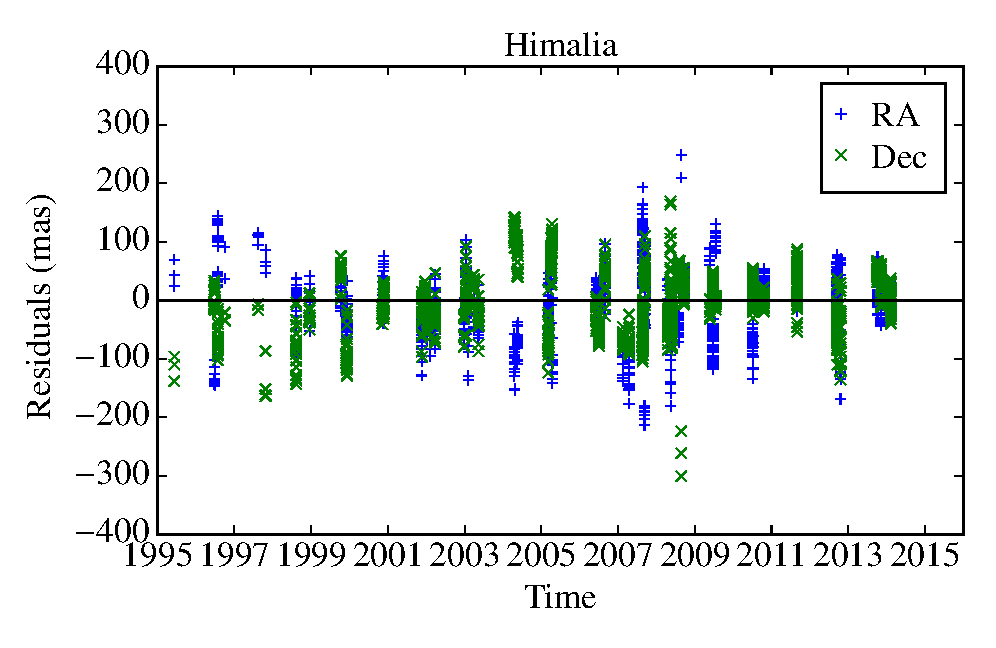
\includegraphics[width=8.8cm]{figures/Himalia_resid.eps}   \label{Fig: residuals-Himalia}}
%\subfigure{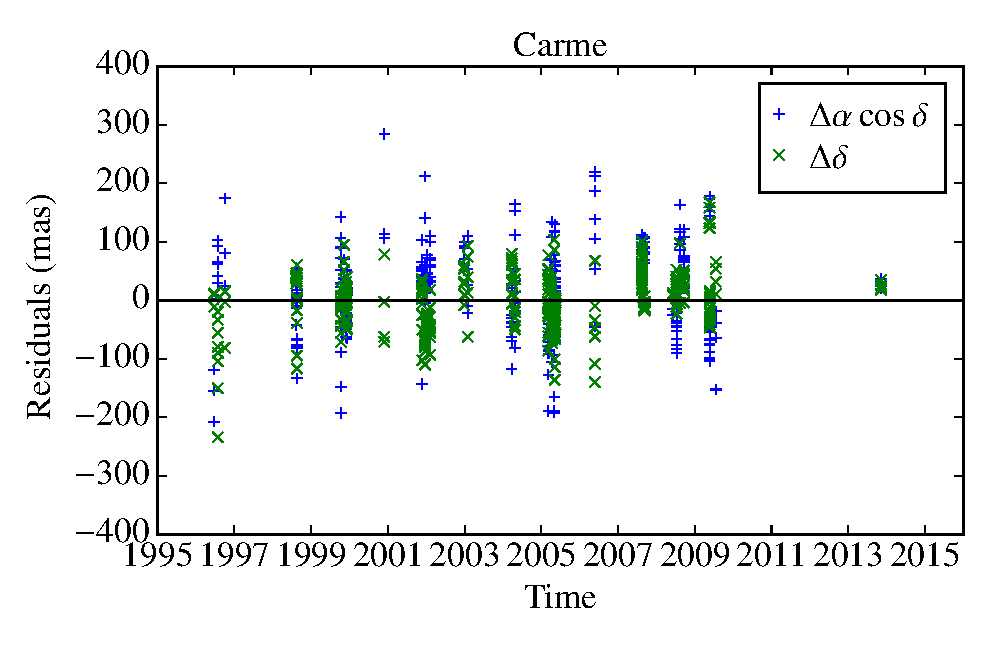
\includegraphics[width=8.8cm]{figures/Carme_resid.eps}  \label{Fig: residuals-Carme}}
%\caption{Residuals in topocentric right ascension and declination of the numerical integration for Himalia and Carme. \label{Fig: residuals}}
%\end{figure*}

%\begin{table*}
%\caption{Initial osculating elements for Jupiter irregular satellites at JD 2451545.0.% For Themisto's case, the small number of observations meant that the statistical uncertainty was even greater than the obtained elements, though the fitting proved satisfying. We decided to provide its elements with significant number comparable to the other satellite for information, but left it without uncertainty.
% }\label{Tab: sat_ell}
%\begin{center}
%\begin{tabular}{ccccccc}
%\hline\hline
%Satellite & a (km) & e & I$\degr$ & $\Omega\degr$ & $\omega\degr$ & $v\degr$ \\ 
%\hline
%Himalia &   11372100 $\pm$ 500    &    0.166 $\pm$ 0.002      &   45.14 $\pm$ 0.15      &   39.77 $\pm$ 0.19      &   351.48 $\pm$ 0.46      &   97.35 $\pm$ 0.48    \\
%Elara &   11741170 $\pm$ 690  &      0.222 $\pm$ 0.002      &   28.64 $\pm$ 0.18      &   68.42 $\pm$ 0.43      &   179.82 $\pm$ 0.56      &   339.08 $\pm$ 0.82  \\
%Lysithea &   11739900 $\pm$ 1300  &      0.136 $\pm$ 0.004      &    51.12 $\pm$ 0.27     &   5.53 $\pm$ 0.52      &   53.0 $\pm$ 1.5      &   318.9 $\pm$ 2.0   \\
%Leda &   11140300  $\pm$ 4300  &     0.173  $\pm$ 0.007     &   16.15  $\pm$ 0.75    &   272.6  $\pm$ 1.7    &   212.2  $\pm$ 3.6          &   218.8  $\pm$ 3.2  \\
%Pasiphae &  23425000  $\pm$ 5000    &     0.379  $\pm$ 0.001       &   152.44 $\pm$ 0.10      &   284.59 $\pm$ 0.21      &   135.96 $\pm$ 0.19      &   236.97 $\pm$ 0.16 \\
%Sinope &   22968800 $\pm$ 5200   &     0.316 $\pm$ 0.002      &   157.76 $\pm$ 0.12      &   256.62 $\pm$ 0.55      &   298.38 $\pm$ 0.55      &   167.57 $\pm$ 0.19    \\
%Carme &   24202924 $\pm$ 4800      &  0.242 $\pm$ 0.001      &   147.13 $\pm$ 0.10      &   154.01 $\pm$ 0.25      &   47.90 $\pm$ 0.29      &   234.41 $\pm$ 0.19  \\
%Ananke &  21683800  $\pm$ 7200  &     0.380 $\pm$ 0.002      &   172.29 $\pm$ 0.20      &   56.9 $\pm$ 1.2      &   123.3 $\pm$ 1.2      &   231.24 $\pm$ 0.21  \\
%%Themisto  & 7393800    &     0.198       &   25.77  &   220.0     &   216.3    &   262.1     \\
%\hline
%\end{tabular} 
%\end{center}
%\textbf{Notes}: a: semimajor axis; e : excentricity; I: inclination relative to the equatorial reference plane J2000; $\Omega$: longitude of the ascending node; $\omega$: argument of periapsis; $v$: true anomaly.
%\end{table*}

All the orbits determined for the satellites show satisfying residuals. %Yet, one of the satellites has a peculiar situation. Its small number of observations in our set means that its orbit is definitely loosely constrained. 
The residuals are smaller than those obtained with JPL ephemeris, which was expected because the accuracy of an ephemeris decreases when we get further from the time of observations. The main risk of divergence over time comes from the possible absence of long-term effects when fitting to a short timespan of observations. If that were the case, our ephemeris would diverge too quickly to be of any use. JPL ephemerides are fitted over all the available observations. As a result, they will diverge less quickly than our own. Though they are no longer precise enough for our use, they remain a precious reference to identify whether our own model presents a quick divergence.

We compared our ephemeris to the JPL for all the Jupiter satellites we fitted, until 2018. For instance, the divergence between 2015 and 2018 is at most 98 mas in $\Delta \alpha \cos \delta$ and 58 mas in $\Delta \delta$ for Himalia and 181 mas in $\Delta \alpha \cos \delta$ and 152 mas in $\Delta \delta$ for Carme.

Fig. \ref{Fig: JPL-STE} displays the offsets of the positions published by \cite{GomesJunior2015} for the satellite Carme in declination relative to our ephemeris, to \cite{Jacobson2012} JUP300 JPL ephemeris and \cite{Emelyanov2008} ephemeris.We see that the systematic JPL ephemeris offsets pointed out by \cite{GomesJunior2015} are reduced with our ephemeris, as expected.

\begin{figure}
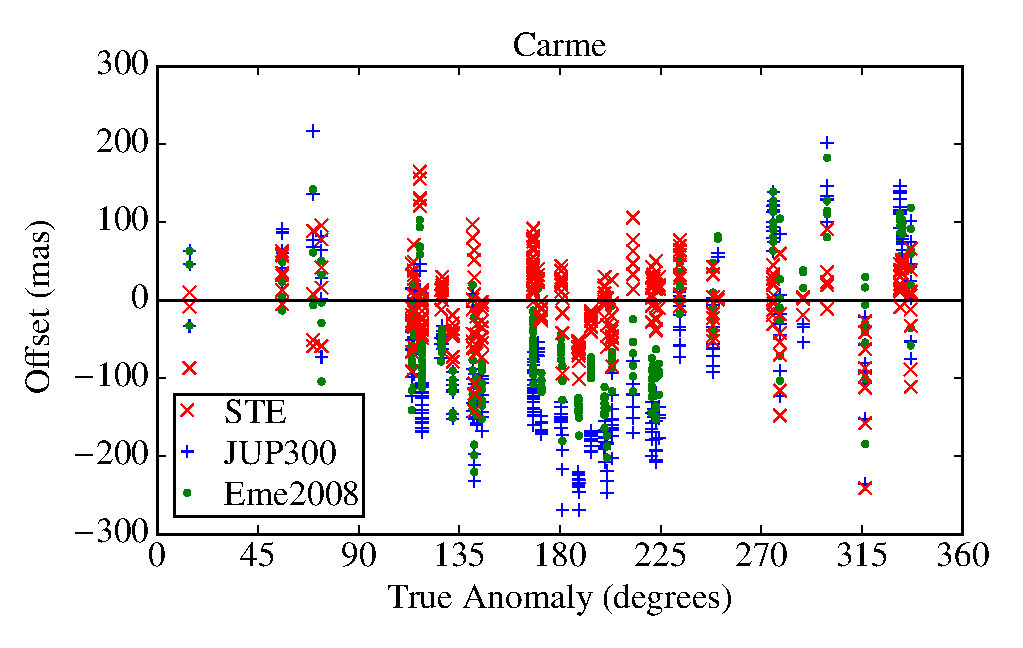
\includegraphics[width=8.8cm]{figures/Carme_ephemeris.eps} 
\caption{Offsets in declination of the positions published by \cite{GomesJunior2015} for Carme. The red "x" relative to the special-tailored ephemeris, the blue "+" relative to the JUP300 JPL ephemeris and the green dot relative to \cite{Emelyanov2008}. As expected, the ephemeris systematic errors pointed out by \cite{GomesJunior2015} are reduced with the STE ephemeris.  \label{Fig:JPL-STE}}
\end{figure}

%\begin{figure*}
%\subfigure{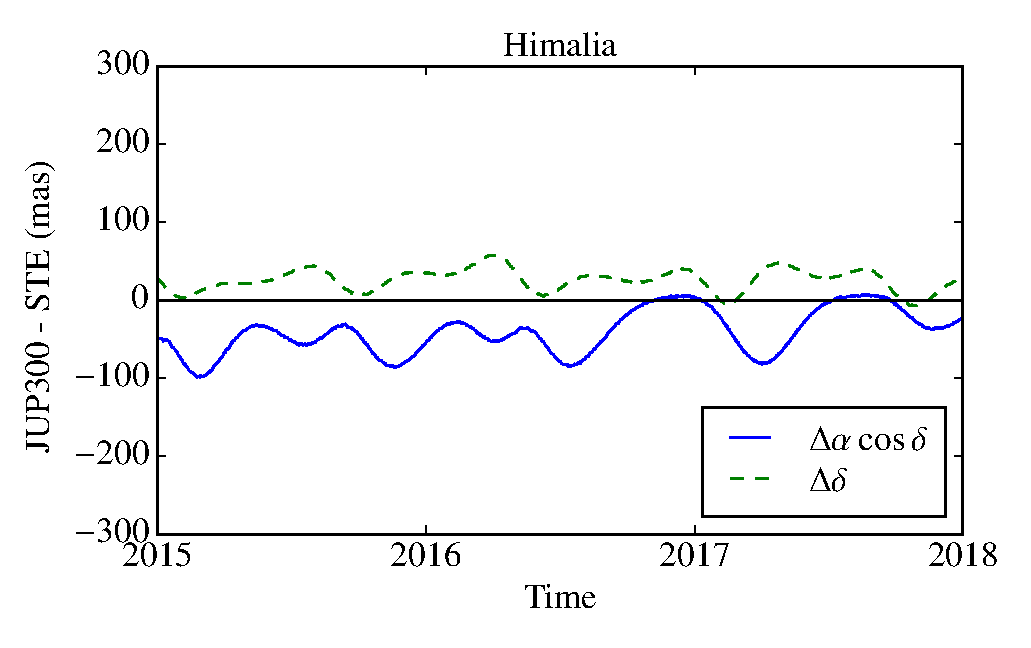
\includegraphics[width=8.8cm]{figures/JPL_DEC_Himalia.eps}    \label{Fig: JPL-STE-Himalia}}
%\subfigure{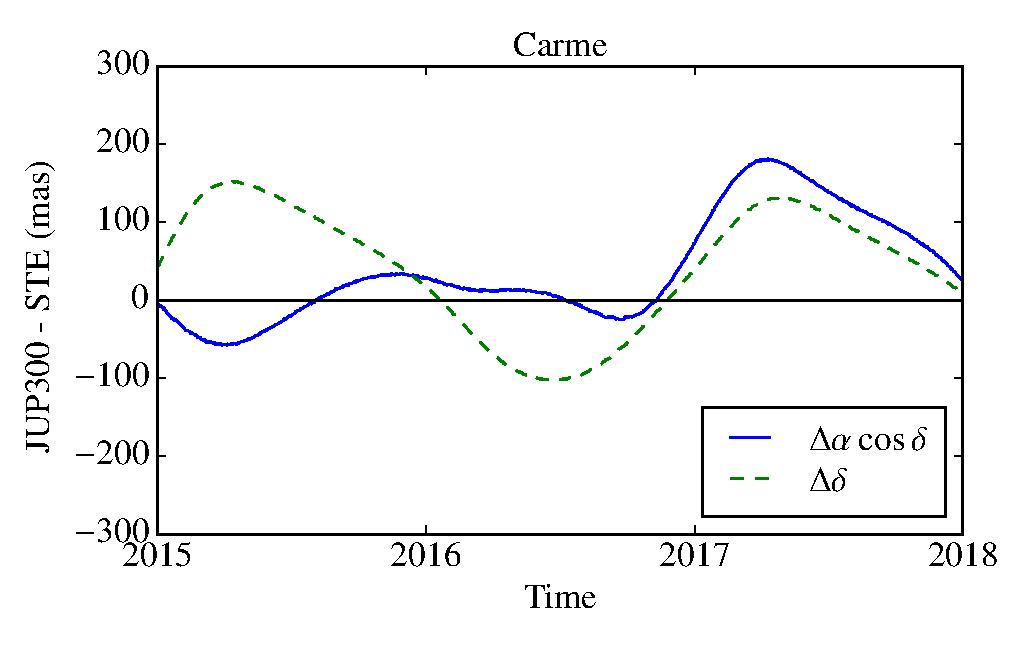
\includegraphics[width=8.8cm]{figures/JPL_DEC_Carme.eps}  \label{Fig: JPL-STE-Carme}}
%\caption{Geocentric right ascension and declination differences between the JUP300 JPL ephemeris and the special-tailored ephemeris for Himalia and Carme. \label{Fig: JPL-STE}}
%\end{figure*}

The obtained ephemeris is hereafter refered as STE, for special-tailored ephemeris.

\subsection{Phoebe's ephemeris}

For the specific case of Phoebe, the ninth satellite of Saturn, we have updated the ephemeris published in \cite{Desmars2013}. The new ephemeris (PH15) used the same dynamical model, including the perturbations of the Sun and the eight planets, the eight major satellites of Saturn and the $J_2$ parameter. The observations used to fit the model are identical to \cite{Desmars2013} (including 223 Cassini observations) with additional observations from \cite{GomesJunior2015}, \cite{Peng2015}, observations from Minor Planet Circulars between 2012 and 2014 (available on the Natural Satellite Data Center\footnote{\url{http://lnfm1.sai.msu.ru/neb/nss/bsapoouf.htm}}), and observations from Flagstaff \citep{NOFS} between 2012 and 2014. It represents a total number of 5886 observations from 1898 to 2014.

In Fig. \ref{Fig:eph-Phoebe} we compare our ephemeris (PH15) with the SAT375 JPL\footnote{Jacobson, R.A. 2015-Feb-27. "Satellite Ephemeris: SAT375", JPL Satellite Ephemeris File Release, \url{ftp://ssd.jpl.nasa.gov/pub/eph/satellites/nio/LINUX_PC/sat375l.txt}} and the \cite{Emelyanov2007} ephemeris. We can see that our ephemeris is closer to the SAT375 JPL ephemeris where the difference between them is smaller than 20 mas (< 10 mas in Declination). This difference is smaller than the apparent diameter of Phoebe (see Table \ref{Tab: satellite-diameter})

\begin{figure}
\begin{centering}
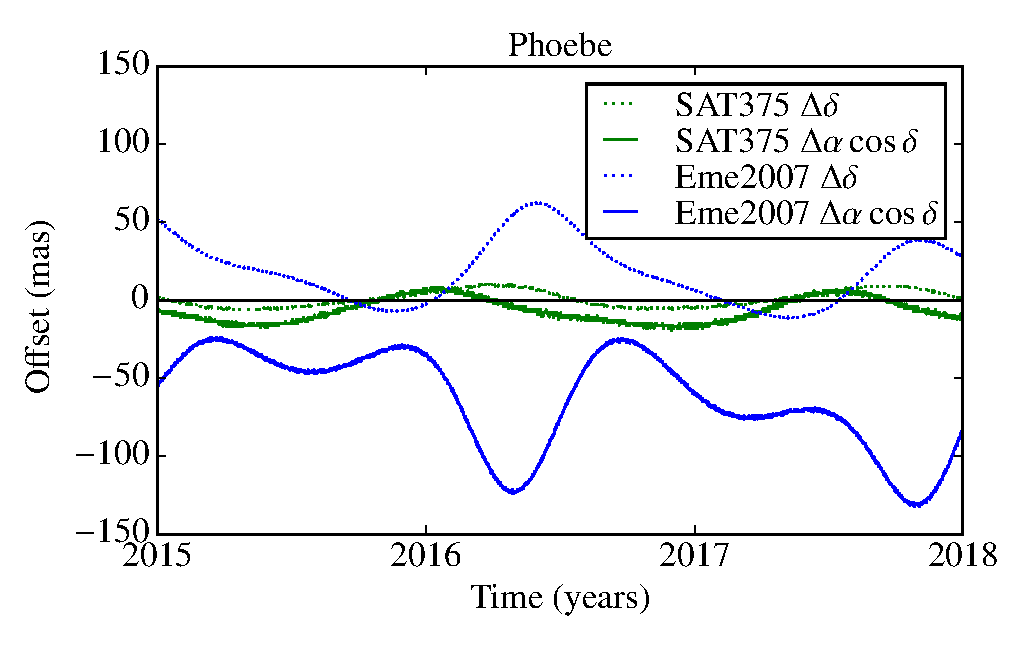
\includegraphics[width=8.8cm]{figures/Phoebe.eps} 
\caption{Comparison between the PH15, SAT375 JPL and \cite{Emelyanov2007} ephemeris for the satellite Phoebe.}
\label{Fig:eph-Phoebe}
\end{centering}
\end{figure}

\subsection{Triton's and Nereid's ephemeris}

For Triton, we used the most recent ephemeris published by \cite{Emelyanov2015}. In Fig. \ref{Fig:eph-Triton} we compare it with the ephemeris published in \cite{Zhang2014} and the NEP081 JPL ephemeris \citep{Jacobson2009}. The offsets between the three ephemeris are smaller than 15 mas for the period 2015-2018. This value is much smaller than the apparent size of Triton (124 mas, see Table \ref{Tab: satellite-diameter}), which indicates a good probability of observing an event by this object.

\begin{figure*}
\begin{centering}
\subfigure[NEP081 JPL and \cite{Emelyanov2015}]{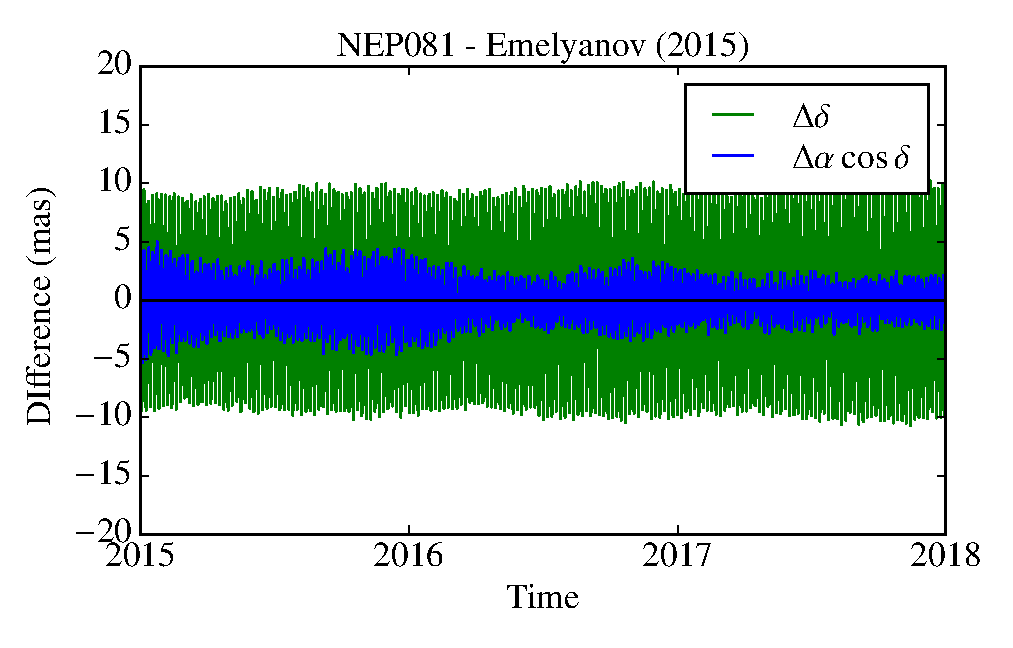
\includegraphics[width=8.8cm]{figures/JPL-EME_Triton.eps} \label{Fig:eph-Triton-eme}}
\subfigure[\cite{Zhang2014} and \cite{Emelyanov2015}]{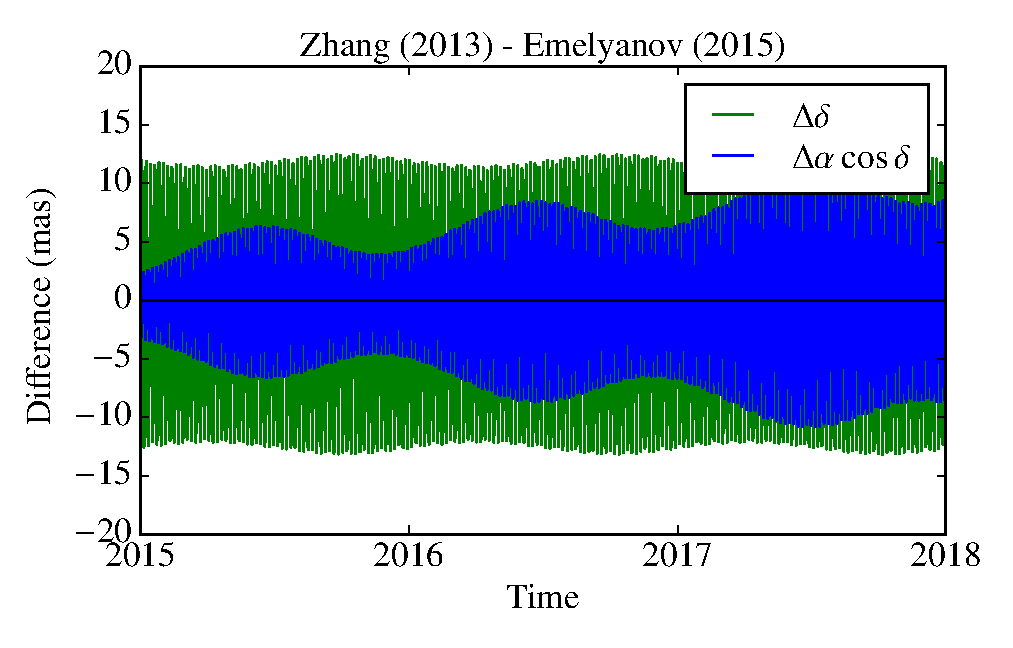
\includegraphics[width=8.8cm]{figures/Zhang-EME.eps} \label{Fig:eph-Triton-zhang}}
\caption{Comparison between the \cite{Emelyanov2015}, \cite{Zhang2014} and NEP081 JPL \citep{Jacobson2009} ephemeris for the satellite Triton.}
\label{Fig:eph-Triton}
\end{centering}
\end{figure*}

For Nereid, we used the ephemeris published by \cite{Emelyanov2011}, which uses more recent observations than the JPL ephemeris published by \cite{Jacobson2009}. The comparison between the two ephemeris can be seen in Fig. \ref{Fig:eph-Nereid}. The right ascension offsets between them are smaller than 60 mas and the declination ones are smaller than 15 mas. For Nereid, ephemeris errors in right ascension translate to uncertainties in the central instant of a stellar occultation, so offsets of 60 mas are not critical. The declination ephemeris offsets are of the order of the apparent diameter (15 mas, see Table \ref{Tab: satellite-diameter}), resulting in fair chances (50\%) that the shadow crosses the expected Earth latitude predicted for an occultation. % which is bigger than the satellite apparent diameter (see Table \ref{Tab: satellite-diameter}). Although this fact, the difference is bigger in Right Ascension than in Declination, which means that, in an event, the error would be smaller in the latitude where the shadow will pass on Earth than the error at the time of the occultation.

\begin{figure}
\begin{centering}
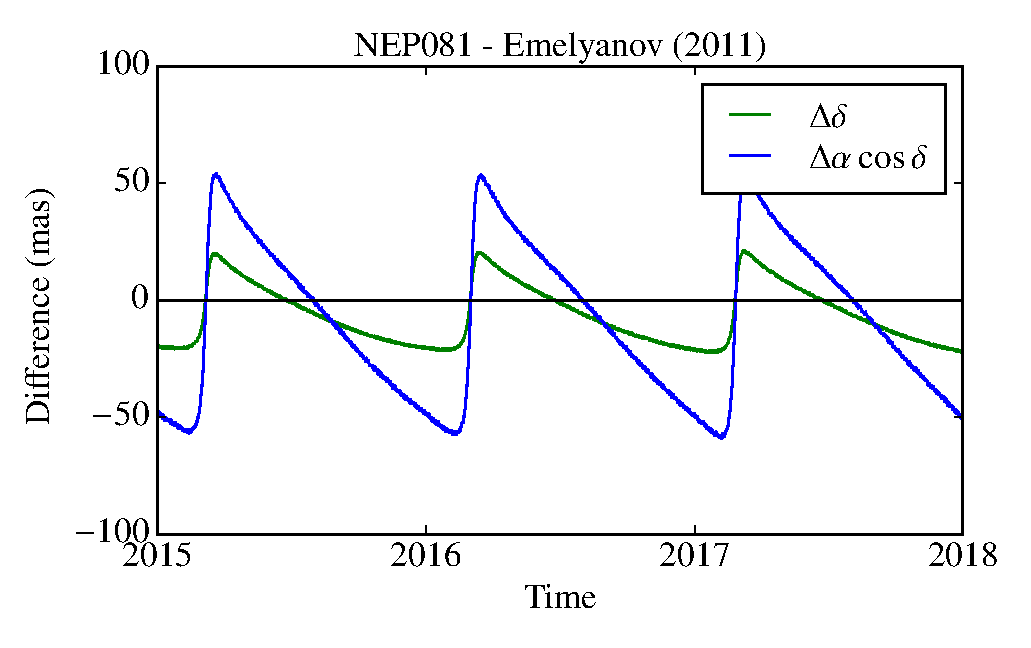
\includegraphics[width=8.8cm]{figures/JPL-EME_Nereid.eps}
\caption{Comparison between the \cite{Emelyanov2011} and NEP081 JPL \citep{Jacobson2009} ephemeris for the satellite Nereid.}
\label{Fig:eph-Nereid}
\end{centering}
\end{figure}

\cite{GomesJunior2015} published 902 new positions for Nereid from observations between 1992 and 2014. The development of a better ephemeris for Nereid using these new positions in the context discussed here of near future stellar occultations is desirable, but is out of the scope of this paper.  

%Making a new model for the orbits of these objects would demand a lot of time and delay the publication of predictions of possible events to occur in the very near future. Thus, we utilized the positions obtained by \cite{GomesJunior2015} to identify error patterns in the ephemeris. The error patterns in right ascension and in declination could be used to extrapolate the offsets to the satellite ephemeris by the time of the predicted occultation, improving it. Plots of the offsets over true anomaly (see Fig. \ref{Fig:offxanom} for declination offsets of Carme, for instance) clearly show the systematic errors in the JPL ephemeris.

%\begin{figure}
%\begin{centering}
%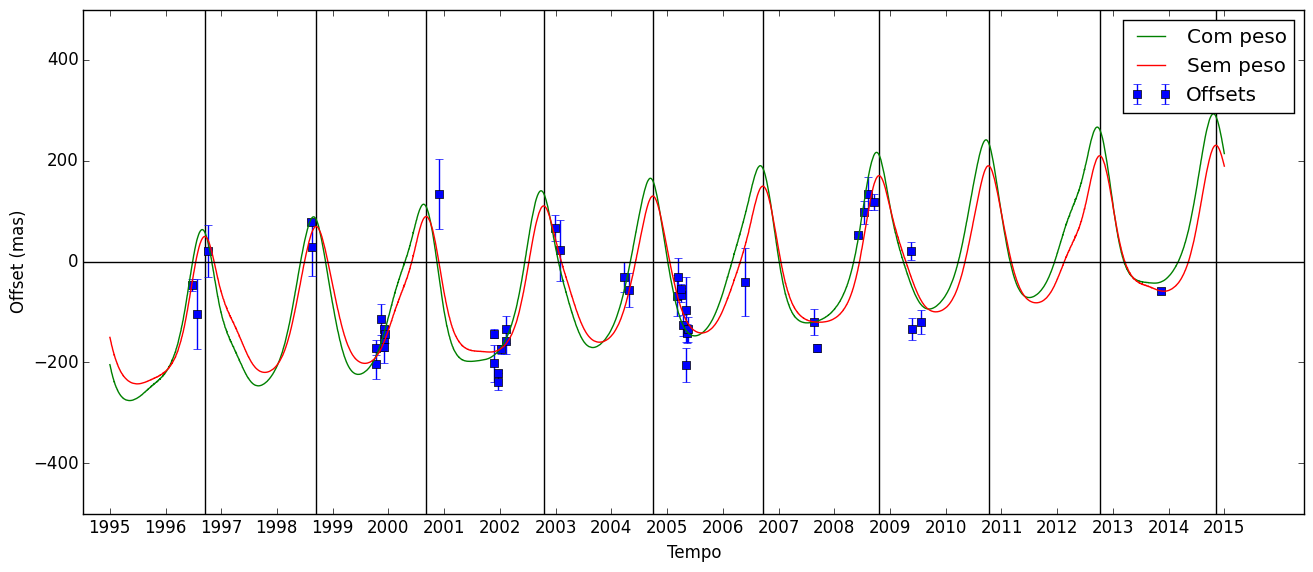
\includegraphics[scale=0.25]{figures/DEC.png}\label{Fig:offxtime}
%\caption{Offsets of the declination of Carme by time. \textcolor{red}{Figura só para visualização, vou colocar alguma melhor depois}}
%\end{centering}
%\end{figure}

%\begin{figure*}
%\begin{centering}
%\subfigure[Offset from the JPL ephemeris]{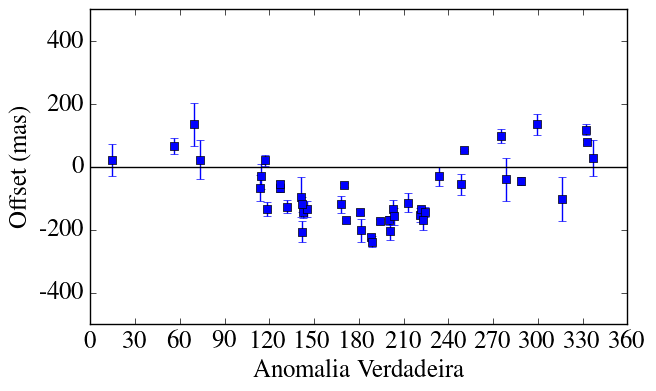
\includegraphics[width=8.8cm]{figures/DEC_anom.png} \label{Fig:offxtanomxjpl}}
%\subfigure[\textcolor{red}{Offset from the numerical integration}]{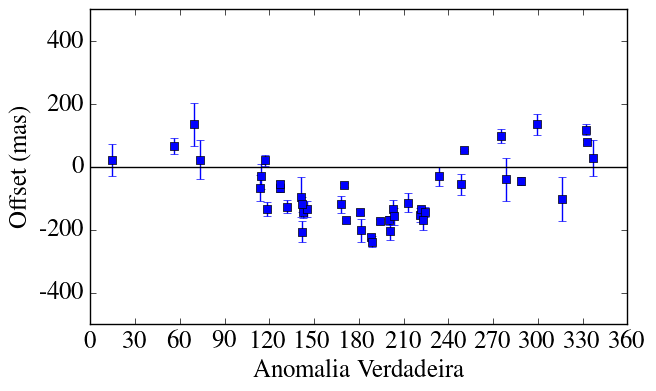
\includegraphics[width=8.8cm]{figures/DEC_anom.png} \label{Fig:offxtanomxni}}
%\caption{Offsets of the declination of Carme by true anomaly from the JPL ephemeris and \textcolor{red}{from the numerical integration of the positions obtained in \cite{GomesJunior2015}}.
%\label{Fig:offxanom}}
%\end{centering}
%\end{figure*}


%The two kinds of error or offset patterns adopted depending on the case are given by Eqs. \ref{eq:linear} and \ref{eq:seno}:
%
%\begin{equation}
%F(t,f) = p[0]\times t + p[1]\times \sin(f) + p[2]\times\cos(f) + p[3],
%\label{eq:linear}
%\end{equation}
%
%\begin{equation}
%\begin{split}
%%F = \{F_{x} \in  F_{c} &: (|S| > |C|) \\
%% &\quad \cap (\text{minPixels}  < |S| < \text{maxPixels}) \\
%% &\quad \cap (|S_{\text{conected}}| > |S| - \epsilon) \}
%F(t,f) = p[0]\times\sin\left(\frac{2\pi}{p[1]}\times t + p[2]\right) + p[3]\times\sin(f) + \\ +p[4]\times\cos(f) + p[5],
%\end{split}
%\label{eq:seno}
%\end{equation}
%where $F(t,f)$ is the offset obtained, $t$ is time in years counting from J2000.0 and $f$ is the true anomaly. The patterns could be applied for right ascension as well as for declination ephemeris offsets.

\section{Prediction of occultations} \label{Sec: predictions}

The prediction of the occultations was made by crossing the stellar coordinates and proper motions of the UCAC4 catalogue \citep{Zacharias2013} with the ephemeris presented in Sec. \ref{Sec: integration}. The search for stellar candidates follows the same procedure as presented by \cite{Assafin2010, Assafin2012} and \cite{Camargo2014}.

We predicted occultations for the 8 major irregular satellites of Jupiter,  Ananke, Carme, Elara, Himalia, Leda, Lysithea, Pasiphae and Sinope, and for Phoebe of Saturn and Triton and Nereid of Neptune.

For Triton and Nereid, the candidates for stellar occultations in 2016 were searched using the WFI catalogue in the same way as the predictions for Centaurs and TNOs occultations by \cite{Assafin2010, Assafin2012} and \cite{Camargo2014}. This catalogue contains the stars in the path of Neptune in the sky up to mid-2016. The catalogue was generated by observations made at the ESO 2p2 telescope (IAU code 809) using the Wide Field Imager (WFI) CCD mosaic detector. The filter used was the broad-band R filter ESO\#844 with $\lambda_c$ = 651.725 nm and $\Delta\lambda$ = 162.184 nm.

A total of 396 events were identified between January 2016 and December 2017. In Table \ref{Tab: satellite-occultation} we present the number of stellar occultations predicted by year for each satellite. Table \ref{Tab: occ-list} shows a sample of the catalogue of occultations generated and their parameters, which are necessary to produce occultation maps. Since these objects are very small, the duration of each event is a few seconds. All the occultation tables and maps will be publicly available at the CDS. No star brighter than MagR*=18 will be occulted by Triton in 2016. For this satellite, we cut events with stars fainter than R=18, since for Triton the flux drop during such an occultation would be very small. In Fig. \ref{Fig: ocultacao} we show an example of an occultation map. This is the only found occultation by Triton and it will happen in October 05, 2017. This event can be observed from Europe and the east coast of USA and will be a great opportunity to study in high resolution the atmosphere of the satellite.

\begin{table}
\caption{\label{Tab: satellite-occultation} Number of stellar occultations for each satellite from January, 2016 up to December, 2017.}
\begin{centering}
\begin{tabular}{lccc}
\hline  \hline
%\multicolumn{4}{c}{Diameter of the satellites} \tabularnewline
Satellite  & 2016 & 2017 & Total \tabularnewline
\hline
Ananke & 12 & 16 & 28 \tabularnewline
Carme & 20 & 14 & 34 \tabularnewline
Elara & 14 & 16 & 30 \tabularnewline
Himalia & 15 & 12 & 27 \tabularnewline
Leda & 8 & 24 & 32 \tabularnewline
Lysithea & 16 & 11 & 27 \tabularnewline
Pasiphae & 20 & 19 & 39 \tabularnewline
Sinope & 15 & 21 & 36 \tabularnewline
\hdashline
Phoebe\tablefootmark{a} & 32 & 98 & 130 \tabularnewline
\hdashline
Nereid\tablefootmark{a} & 11\tablefootmark{b} & 1 & 12 \tabularnewline
Triton\tablefootmark{a} & -- & 1 & 1 \tabularnewline
\hline
\end{tabular}
\par \end{centering}
Occultations predicted using the UCAC4 catalogue and STE ephemeris.
\tablefoottext{a}{Using JPL ephemeris.}
\tablefoottext{b} {Using the WFI catalogue as explained in Sec. \ref{Sec: predictions}}.
\end{table}

\begin{table*}
\caption{\label{Tab: sample-cds} A sample of stellar occultation predictions for Pasiphae}
\begin{centering}
\begin{tabular}{cccrcccrcrr}
\hline
\hline
d m Year~~~~h~~m~~~s & RA~~~(ICRS)~~~Dec & C/A & P/A & $\nu$ & {\it D} & $R^*$ & $\lambda$ & LST & $\mu_{\alpha*}$ & $\mu_{\delta}$ \tabularnewline
\hline
% & \multicolumn{2}{c}{Mean errors} & Nr & Nr &  UCAC4       \tabularnewline
09 04 2016 03:58:19. & 11 14 36.7707 +07 39 20.7610 & 1.003 &  17.9 & -12.88 &  4.54 & 14.9 & 271. & 22:03 &  12. & -33. \tabularnewline 
13 06 2016 00:16:12. & 11 12 48.5020 +07 06 43.3520 & 0.661 &  30.0 & +14.32 &  5.50 & 13.9 & 262. & 17:45 &  -1. &   1. \tabularnewline 
27 06 2016 13:56:09. & 11 18 03.4160 +06 23 45.1940 & 1.707 &  28.0 & +20.29 &  5.74 & 11.7 &  44. & 16:53 &   4. & -10. \tabularnewline 
18 07 2016 15:07:24. & 11 28 15.5076 +05 05 31.8060 & 0.942 &  26.7 & +27.80 &  6.05 & 14.0 &   8. & 15:40 &   4. &   4. \tabularnewline 
22 07 2016 16:15:07. & 11 30 30.4310 +04 48 43.4340 & 0.644 & 206.5 & +29.04 &  6.11 & 14.6 & 348. & 15:27 &  23. & -24. \tabularnewline 
24 07 2016 01:37:34. & 11 31 17.8471 +04 42 49.0540 & 0.029 & 206.6 & +29.46 &  6.12 & 15.1 & 206. & 15:22 &   2. &  -8. \tabularnewline 
24 07 2016 17:37:18. & 11 31 40.7472 +04 39 57.5060 & 0.840 &  26.5 & +29.66 &  6.13 & 14.9 & 326. & 15:20 & -11. &  -1. \tabularnewline 
\hline
\end{tabular}
\par\end{centering}
\textbf{Notes}. Entries included: day of the year and UTC time of the prediction; right ascension and declination of the occulted star - at the central instant of occultation (corrected by proper motions); C/A: the geocentric closest approach, in arcseconds; P/A: the satellite position angle with respect to the occulted star at C/A, in degrees (zero at north of the star, increasing clockwise); $\nu$: velocity in the plane of sky, in km s$^{-1}$: positive = prograde, negative = retrograde; {\it D}: planet range to Earth, in AU; $R^*$: normalized magnitude to a common shadow velocity of 20 km s$^{-1}$ by the relationship $\textrm{R}^* = \textrm{R}_{\textrm{actual}} + 2.5 \times \log 10 \left(\frac{\textrm{velocity}} {20 \textrm{km}\, \textrm{s}^{-1}} \right)$; $\lambda$: east longitude of subplanet point in degrees, positive towards east; LST: UT + $\lambda$: local solar time at subplanet point, hh:mm; $\mu_{\alpha *}$ and $\mu_{\delta}$: proper motions in right ascension and declination, respectively (mas/year).
\label{Tab: occ-list}
\end{table*}

\begin{figure*}
\begin{centering}
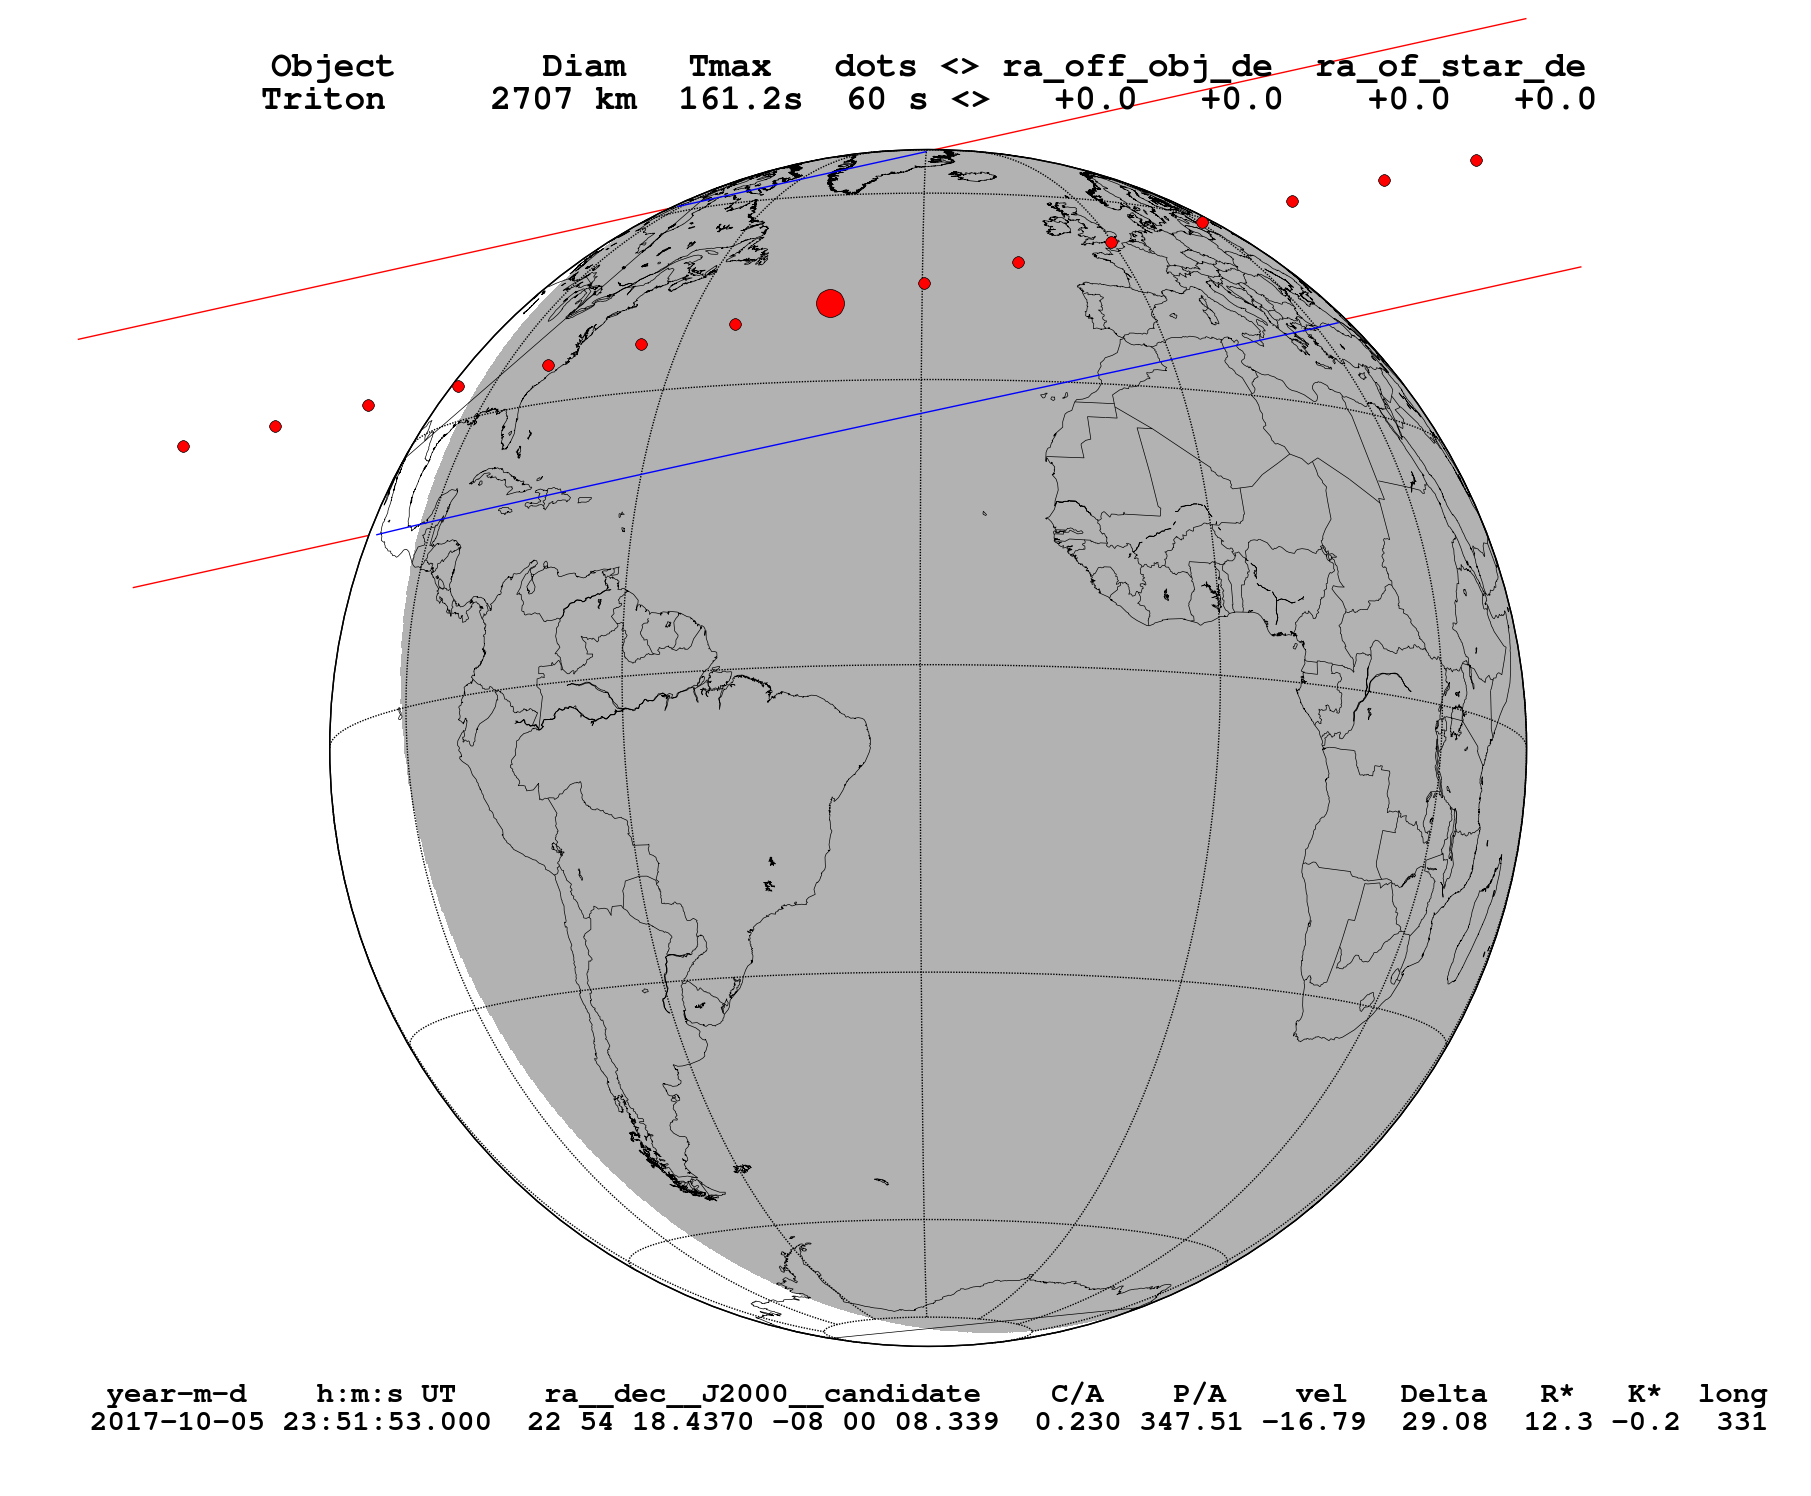
\includegraphics[scale=0.4]{figures/Triton_2017-10-05T23:51:53.png}   
\caption{Occultation map for Triton.% regarding to the first event sampled in Table \ref{Tab: occ-list}.
The central red dot show the geocentric closest approach of the shadow. The small ones shows the center of the shadow separated by 60s. The lines show the path of the shadow over the Earth. The shadow moves from right to left.
\textbf{Labels:} Diam: Diameter of the object; Tmax: Maximum duration of the event for a central observation; C/A: the geocentric closest approach, in arcseconds; P/A: the satellite position angle with respect to the occulted star at C/A, in degrees; vel: velocity of event in km/s; Delta: Geocentric distance to the occulting object in AU; $R^*$: normalized magnitude to a common shadow velocity of 20 km s$^{-1}$; long: east longitude of subplanet point in degrees, positive towards east.}
\label{Fig: ocultacao}
\end{centering}
\end{figure*}

The first preliminary catalogue version of the ESA astrometry satellite GAIA \citep{deBruijne2012} is expected to be released up to the end of 2016. The precise star positions to be derived by GAIA will provide better predictions with the main source of error being the ephemeris. Astrometric reduction of observations published in \cite{GomesJunior2015} will be revised with the GAIA catalogue and the predictions from 2017 onwards will be improved. Since we cannot foresee exactly when the GAIA catalogue will be released and when new and re-reduced satellite positions in the GAIA frame will become available, we decided to publish only the predictions for occultations restricted to the 2016-2017 time interval.


\section{Occultation test} \label{Sec: testes}

Observing a stellar occultation demands a great effort. And, in our case, the shadow covers a very restricted area on Earth because of the size of the irregular satellites. Since no stellar occultation by an irregular satellite was observed up to date, with the exception of Triton, and since we want to be sure that we can start observational campaigns with reasonable chances of success, we tested an occultation prediction for a large target, to assess the quality of the prediction.

The test design consisted in observing the object and star to be occulted near the date of the event predicted when the two objects were present in the same field of view (FOV), close to each other. Thus, the relative positions between the two objects had minimal influence of the errors of the reference catalogue of stars used and possible field distortions \citep[and references therein]{Peng2008}. The relative positions of the star and satellite were used to check the original predictions. Notice that in the test we do not attempt to observe any actual occultation. The test could be performed at any site, regardless of the Earth location where the occultation would in fact be visible. 

We tested the occultation by Himalia predicted to occur on March 3, 2015. The shadow would cross the northern part of South America. For the event, four situations were considered:
\begin{enumerate}[I]
\item Our nominal, published prediction with the STE ephemeris (see Sec. \ref{Sec: integration}), and the nominal UCAC4 position of the star;
\item Prediction with the JPL ephemeris and the nominal UCAC4 position of the star;
\item From star and satellite offsets calculated from observations made a few days before the occultation when the objects were very separated (different FOVs);
\item Same as 3 but with the star and the satellite close in the same FOV.
\end{enumerate}

Table \ref{Tab: comparison-Himalia} shows the differences between the predictions in the four situations. For situation 3 we observed the objects on February 22 with the Zeiss telescope (diameter = 0.6m; FOV = $12\farcm6$; pixel scale = $0\farcs37 / pixel$) at the Observatório do Pico dos Dias, Brazil (OPD, IAU code 874, 45\degr 34\arcmin 57\arcsec W, 22\degr 32\arcmin 04\arcsec S, 1864m). On that day, Himalia and the star were observed in separate FOVs as they were still far apart. On the night of the event, March 3, the objects were observed with Perkin-Elmer telescope (diameter = 1.6m; FOV = $5\farcm8$; pixel scale = $0\farcs17 / pixel$) at OPD just over an hour after the time scheduled for the event. Satellite and star were separated by about 16 arcsec, so very close to each other (situation 4). From the calculated offsets, the center of the shadow was obtained. Notice that the shadow path was not predicted to cross the OPD (which was located at almost 2000 km south from the shadow path). This was not necessary for testing the prediction.

%\begin{figure*}
%\begin{centering}
%\subfigure[Prediction with STE ephemeris]{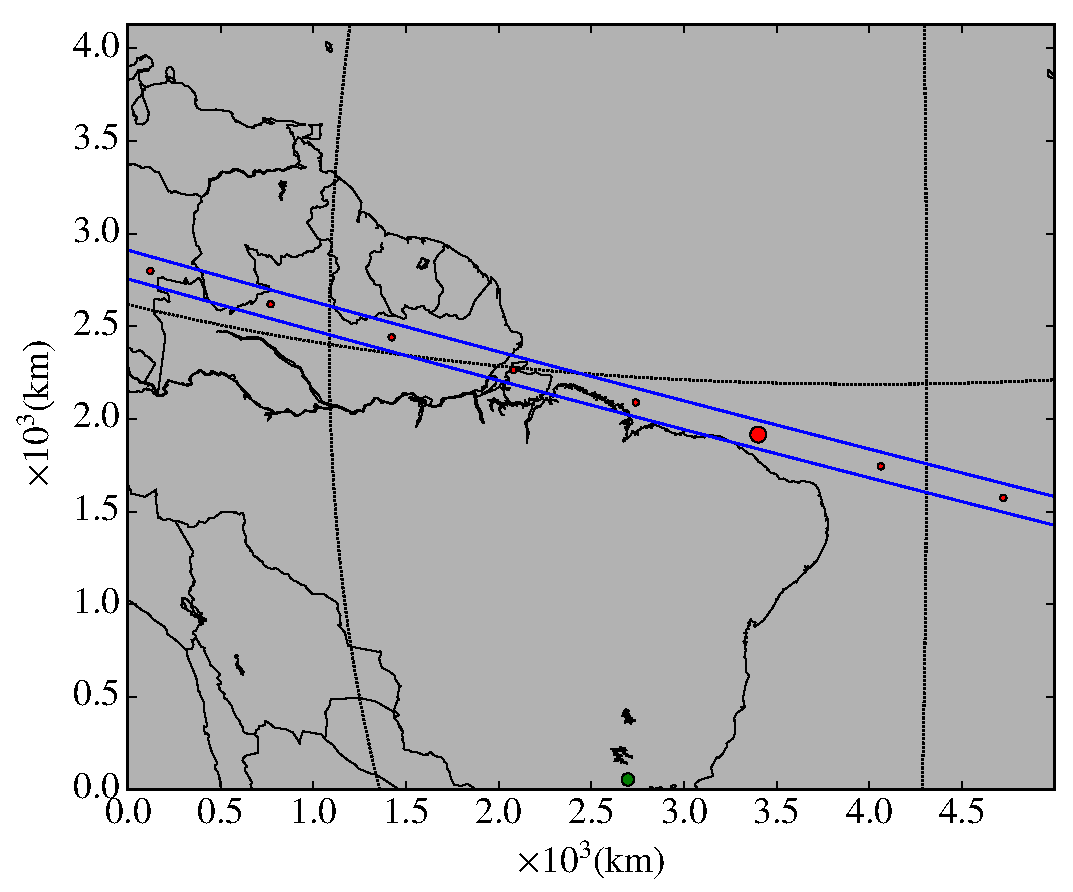
\includegraphics[width=8.8cm]{figures/Himalia_STE.eps}  \label{Fig: occ-Himalia-STE}}
%\subfigure[Prediction with JPL ephemeris]{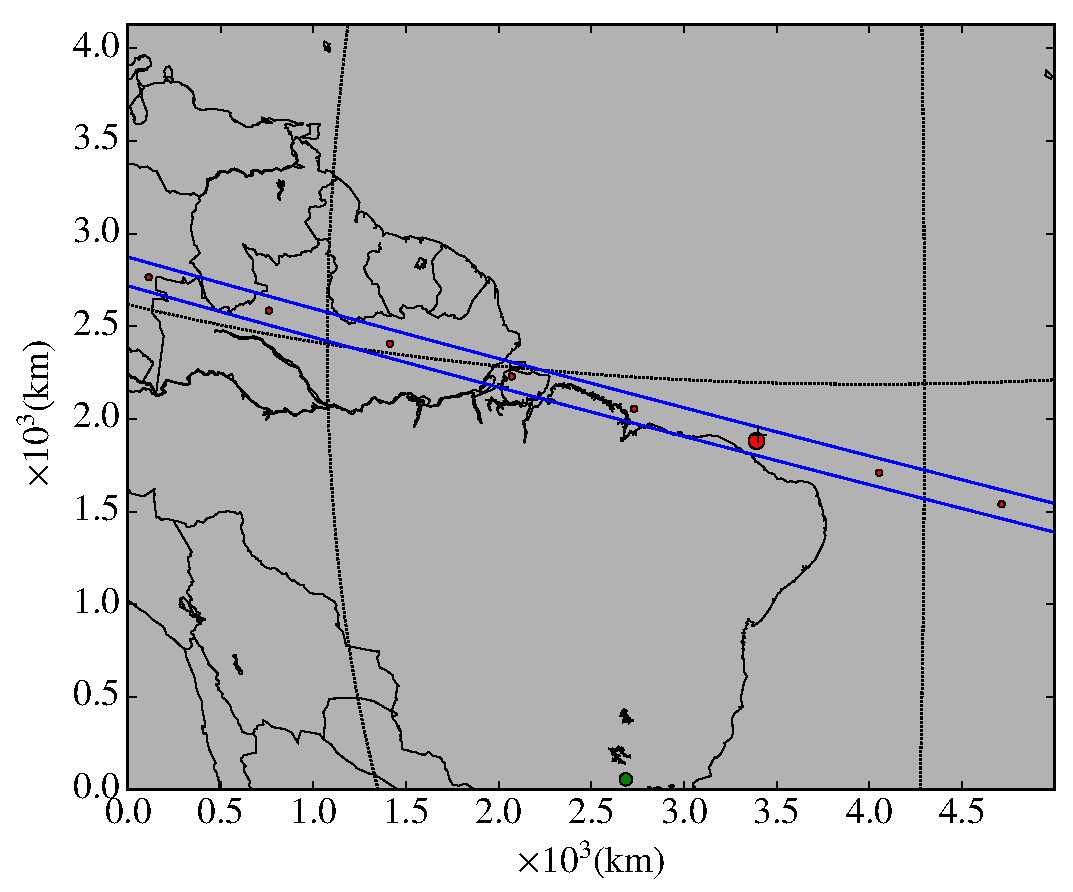
\includegraphics[width=8.8cm]{figures/Himalia_JPL.eps}  \label{Fig: occ-Himalia-JPL}}
%\subfigure[Observation at February 22 (different FOVs)]{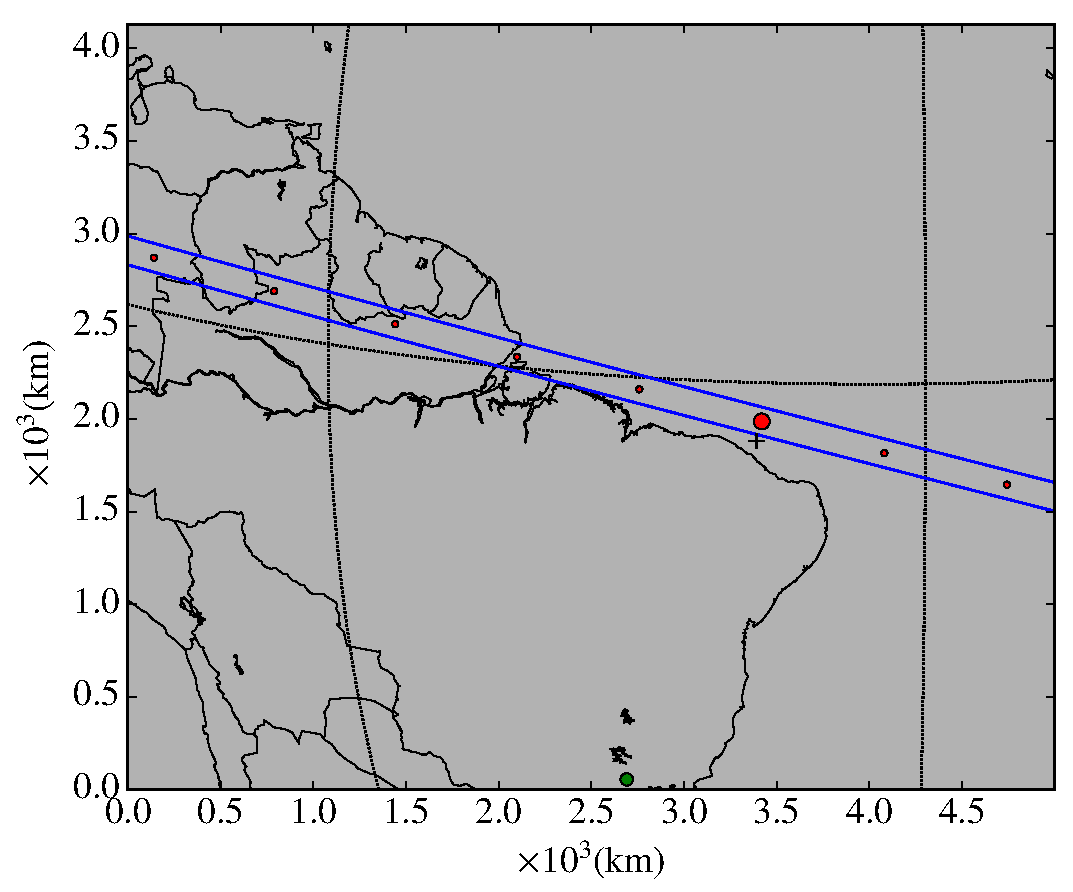
\includegraphics[width=8.8cm]{figures/Himalia_22fev.eps}   \label{Fig: occ-Himalia-off22fev}}
%\subfigure[Observation at March 03 (same FOV)]{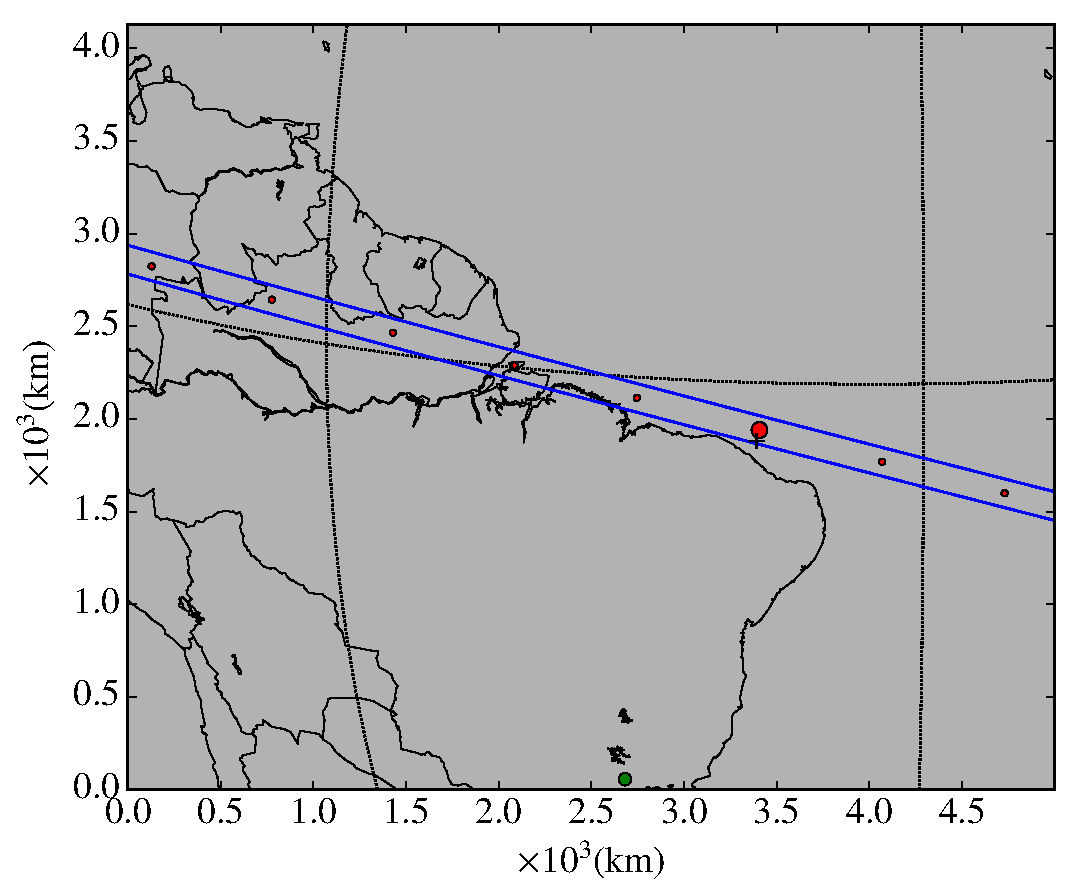
\includegraphics[width=8.8cm]{figures/Himalia_03mar.eps}   \label{Fig: occ-Himalia-off03mar}}
%\caption{Predictions for Himalia: The straight lines show the size of the shadow. The big red dot show the geocentric closest approach of the shadow. The black "+" marks at maps (b,c,d) are the STE prediction closest approach for reference. The small red ones are the center of the shadow separated by one minute. \ref{Fig: occ-Himalia-STE} is the map using the STE ephemeris showed in Sec. \ref{Sec: integration}. \ref{Fig: occ-Himalia-JPL} shows the shadow using the JPL ephemeris. In \ref{Fig: occ-Himalia-off22fev} we apply offsets to the positions of star and satellite accordingly the observations made at February 22. \ref{Fig: occ-Himalia-off03mar} is as in \ref{Fig: occ-Himalia-off22fev} but with observations made at March 03 when the objects were close to each other. The green dot at the bottom of the maps is the location of Observatório do Pico dos Dias.}
%\label{Fig: occ-Himalia}
%\end{centering}
%\end{figure*}

%\begin{figure*}
%\begin{centering}
%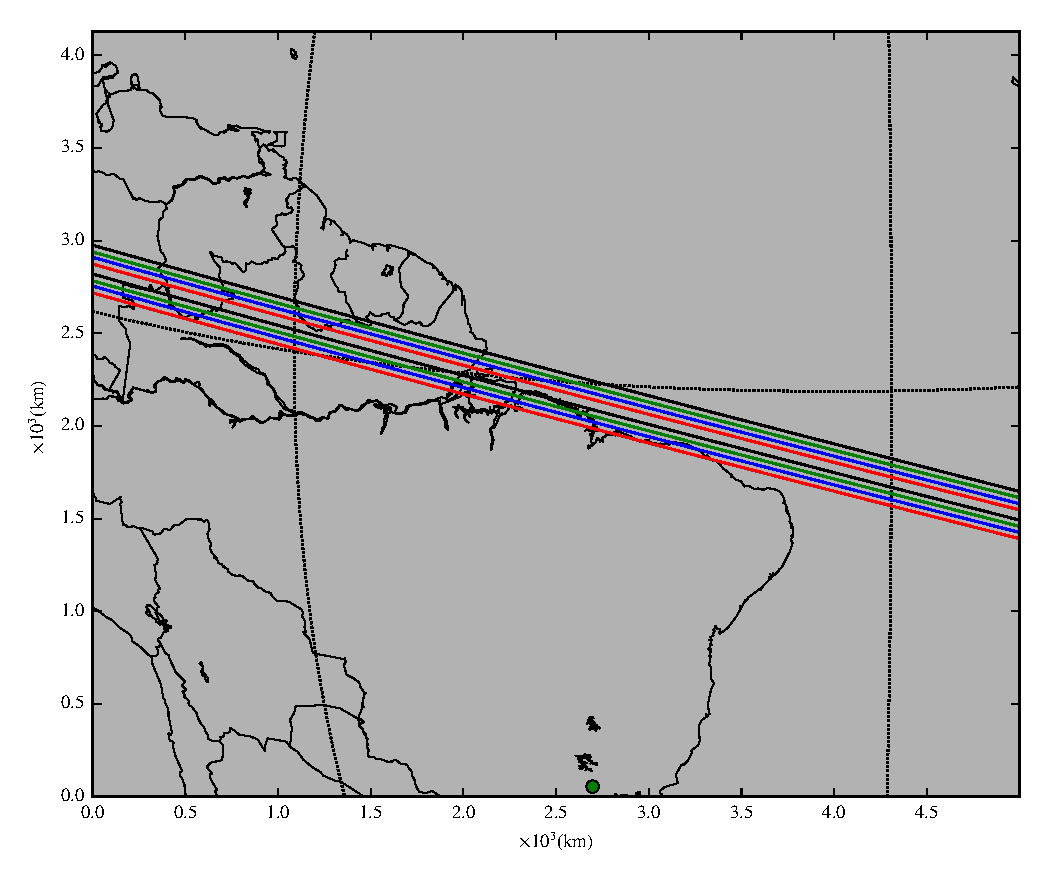
\includegraphics[width=17.6cm]{figures/HIMALIA.eps}
%\caption{Predictions for Himalia: The straight lines show the center of the shadow over time. In blue is for the prediction using the STE ephemeris showed in Sec. \ref{Sec: integration}. In red the shadow using the JPL ephemeris. In black we apply offsets to the positions of star and satellite accordingly the observations made at February 22. In green, the same for the previous one but with observations made at March 03 when the objects were close to each other. The dots show the closest approach of the shadow for each prediction. The scales are relative to the closest approach of the prediction using the STE ephemeris. The bars show the estimated diameter of the satellite and estimated error of the prediction.}
%\label{Fig: occ-Himalia}
%\end{centering}
%\end{figure*}

The critical parameter in the comparisons is the C/A, which here is related to latitudes. The apparent radius of Himalia is about 20 mas (see Table 1). In the context of the test, for a 0 mas offset in C/A we would have 100\% probability of observing the occultation, and 0\% in the case of a C/A offset equal to or larger than 20 mas, the radius of Himalia. From Table 5, we have nearly 0\% probability of success in situation 3, for which the offset in C/A was -20 mas, but when the relative astrometry was poor, 10 days prior to the event. Once at the day of the event in situation 4, the C/A offset dropped to -9 mas only, corresponding to a 55\% probability of success. Comparison with the prediction using the JPL ephemeris (situation 2) gives a +11 mas C/A offset, or a compatibility of 45\% between the ephemerides. All this suggests that there was a good probability of observing the event. The largest differences between the shadows of the four situations were 36s in time along the shadow path and 101km (31 mas) in the direction perpendicular to the shadows, suggesting that observers should be spread in narrow latitude ranges 100 km wide.

\begin{table}
\caption{\label{Tab: comparison-Himalia} Comparison between the predictions of the Himalia occultation at March 03, 2015.}
\begin{centering}
\begin{tabular}{lccc}
\hline  \hline
\multicolumn{4}{c}{Differences with respect to the STE prediction} \tabularnewline
Method  & Instant of C/A  & C/A & Sit.   \tabularnewline
\hline
STE & 00:39:51 UTC & $0\farcs703$ & I \tabularnewline
JPL & -26s & +11mas (36km) & II \tabularnewline % (284km)
Feb. 22 Obs. & -14s & -20mas (65km) & III \tabularnewline % (153km)
Mar. 03 Obs. & -36s & -09mas (29km) & IV \tabularnewline % (393km)
\hline
\end{tabular}
\par\end{centering}
C/A: geocentric closest approach; Sit: Situation test considered.
\end{table}

%The second test was with the satellite Elara, which is the second largest irregular satellite of Jupiter. The event was predicted to occur at March 30, 2015. The observations were made on March 25 and April 2, 2015 with the Zeiss telescope. On the night of April 2 the star and satellite could still be observed in the same FOV. Due to Elara being fainter than Himalia by 2 magnitudes, dispersions of the satellite positions on both nights ended up being higher than for Himalia. %Still, the differences between the maps obtained were relatively small. 
%The largest differences between them were 144s (186 mas) in time along the shadow path and 525 km (153 mas) perpendicular to it (see table \ref{Tab: comparison-Elara}).

%\begin{table}
%\caption{\label{Tab: comparison-Elara} Comparison between the predictions of Elara occultation at March 30, 2015.}
%\begin{centering}
%\begin{tabular}{lcc}
%\hline  \hline
%\multicolumn{3}{c}{Difference from STE prediction} \tabularnewline
%Method  & Instant of C/A  & C/A  \tabularnewline
%\hline
%STE & 01:45:13 UTC & $1\farcs082$ \tabularnewline
%JPL & +02s & +57mas(195km) \tabularnewline
%Mar. 25 Obs. & -70s & +20mas (68km) \tabularnewline
%Apr. 02 Obs. & +74s & -96mas (330km) \tabularnewline
%\hline
%\end{tabular}
%\par\end{centering}
%\end{table}

\section{Discussion} \label{Sec: discussion}

We predict stellar occultations for the period of 2016-2017 for eight irregular satellites of Jupiter: Ananke, Carme, Elara, Himalia, Leda, Lysithea, Pasiphae, and Sinope; one satellite of Saturn: Phoebe; and two satellites of Neptune: Triton and Nereid. The procedure used was the same as that for the prediction of stellar occultations by Pluto and its satellites in \cite{Assafin2010} and by Centaurs and TNOs in \cite{Assafin2012} and \cite{Camargo2014}.

The candidate stars were searched in the UCAC4 catalogue, except for the candidates in 2016 for Triton and Nereid. In this case, we used the WFI catalogue that was generated from observations made with ESO2p2/WFI CCD mosaic that covered the path of Neptune in the sky-plane up to 2016 (see Sec. \ref{Sec: predictions}). From this, a total of 396 events are foreseen. 

In a broader, general sense, the probability of successfully observing an occultation is roughly the ratio of the satellite's radius by the budget error (2 sigma for a 95\% confidence level) of ephemeris and star position. Thus, UCAC4 errors ranging between 20 mas - 50 mas (1 sigma) combined with a mean error (1 sigma) in the JPL ephemeris of 30 mas for Himalia and 150 mas for Leda published in Table 2 of \cite{Jacobson2012} would give 28\%-17\% probability of observing such an event by Himalia and $\approx2$\% for Leda, the smallest irregular satellite in the sample. Observations a few days before the date of occultation predicted may improve the combined errors to 40-80 mas, depending on the magnitude of the objects.

The test made with an occultation expected to happen in March 03, 2015 for Himalia showed that this event would probably have been observed successfully in case there were observers available in the shadow area. %Fig. \ref{Fig: occ-Himalia} shows the maps made for 4 different offset corrections as explained in Sec. \ref{Sec: testes}. Table \ref{Tab: comparison-Himalia} shows numerically the difference between the maps.
%A similar test was made for an occultation of Elara in March 30, 2015. %The difference between the maps in this case are listed in Table \ref{Tab: comparison-Elara}.
The results show satisfying small offsets with respect to the local of the prediction. %We can expect similar results for other satellites and our method should allow successful stellar occultation.

Continuous observations of the satellites are recommended and fitting of our dynamical model to those observations are expected to reduce the respective STE ephemeris errors. The first version of the GAIA catalogue is to be released up to the end of 2016 and will improve the position error of the stars to the 1-5 mas level. It will allow for the discovery of ocultations by fainter stars not present in the UCAC4 catalogue. % Consequently, the astrometry of the satellites with the GAIA catalogue will improve the position errors allowing for better predictions and a higher probabilities of observing stellar occultations by irregular satellites.
The release of the GAIA catalogue should have a positive impact on both the astrometric precision of occulted stars and the reduction of astrometric positions of the satellites. As a result, prediction of stellar occultations by irregular satellites shall increase in number as well as in success.

%We managed a large database with FITS images acquired by 5 telescopes in 3 sites between 1992 and 2014. From that, we identified 8466 observations of irregular satellites, from which we managed to obtain 6523 suitable astrometric positions, giving a total of 3666 positions for 12 satellites of Jupiter, 1920 positions for 4 satellites of Saturn, 35 positions for Sycorax (Uranus) and 902 positions for Nereid (Neptune).

%The positions of all the objects were determined using the PRAIA package. The package was suited to cope with the huge amount of observations and the task of identifying the satellites within the database. PRAIA tasks were also useful to deal with the missing or incorrect coordinate and time stamps present mostly in the old observations.The UCAC4 was used as the reference frame. Based in the comparisons with ephemeris, we estimate that the position errors are about 60 mas to 80 mas depending on the satellite brightness.

%For some satellites the number of positions obtained in this work is comparable to the number used in the numerical integration of orbits by the JPL \citep{Jacobson2012} (see Table \ref{Tab: comparison-horizons}). For instance, the amount of new positions for Himalia is about 70\% of the number used in the numerical integation of orbits by JPL. Systematic errors in the ephemeris were found for at least some satellites (Ananke, Carme, Elara and Pasiphae). In the case of Carme, we evidenced an error in the orbital inclination (see Fig. \ref{Fig: carme_anom}).

%The positions derived in this work can be used in new orbital numerical integrations, generating more precise ephemerides. Stellar occultations by irregular satellites could then be better predicted. Based in this work, our group has already computed occultation predictions for the 8 major irregular satellites of Jupiter. These predictions will be published in a forthcoming paper.


%\begin{acknowledgements}
%
%ARG-J thanks the financial support of CAPES.
%MA thanks the CNPq (Grants 473002/2013-2 and 308721/2011-0) and FAPERJ (Grant E-26/111.488/2013).
%RV-M thanks grants: CNPq-306885/2013, Capes/Cofecub-2506/2015, Faperj/PAPDRJ-45/2013.
%JIBC acknowledges CNPq for a PQ2 fellowship (process number 308489/2013-6).
%BEM thanks the financial support of CAPES.
%FB-R acknowledges PAPDRJ-FAPERJ/CAPES E-43/2013 number 144997, E-26/101.375/2014.
%The numerical model of the satellites of Jupiter was developped during a post-doctoral contract funded by the Chinese Academy of Sciences (CAS) and supported by the National Scientific Fund of China (NSFC)
%
%\end{acknowledgements}

%\begin{thebibliography}{99}
%\bibliography{references.bib}
%\end{thebibliography}
%
%\label{lastpage}

\end{document}
